%======================================================================
\chapter{Deliverables}
%======================================================================

This chapter presents the main deliverables produced by the BorBann project. Since BorBann is a multi-page platform rather than a single demo screen, the delivered outputs include several user-facing workflows, backend and AI services, evaluation assets, and deployment materials. Each deliverable is intended to support a specific part of the real estate analysis process, from account access and property exploration to valuation, location intelligence, and operational monitoring.

The implementation encompasses 11 user interface routes, comprising 2 public and 9 authenticated access points. The system architecture includes 15 backend testing modules, a continuous integration pipeline, and a comprehensive data foundation processing over 800,000 spatial records (points of interest, transit stops, real estate records, and demographic grid cells). This demonstrates a fully functional, production-ready system.

%----------------------------------------------------------------------
\section{Overview of Delivered Outputs}
%----------------------------------------------------------------------

Table \ref{tab:chapter7-overview} groups the delivered outputs by their practical role in the platform. It shows that the final scope includes both user-visible workflows and the supporting technical assets required to keep those workflows reliable.

\begin{table}[htbp]
    \centering
    \small
    \renewcommand{\arraystretch}{1.25}
    \begin{tabularx}{\textwidth}{>{\raggedright\arraybackslash}p{0.21\textwidth}>{\raggedright\arraybackslash}p{0.18\textwidth}>{\raggedright\arraybackslash}X}
        \toprule
        \rowcolor[gray]{0.9} \textbf{Deliverable Group} & \textbf{Main Form} & \textbf{Scope of Delivery} \\
        \midrule
        User access module & Public pages & Login and registration workflows for controlled platform access. \\
        Property exploration module & Main authenticated pages & Interactive map, filters, legends, overlays, property popups, and district-based browsing. \\
        Property detail module & Detail pages & Detailed property and listing pages with map context, nearby properties, and location intelligence. \\
        Valuation module & Wizard and report pages & Input form, location picker, AI valuation report, explainable factors, comparables, and downloadable report. \\
        Chat and guided analysis module & Session pages & AI chat interface with session flow, map context, references, and tool-assisted answers. \\
        Location intelligence module & Analytics layer & Livability scoring, transit access, walkability metrics, and risk assessment indicators. \\
        Market analytics module & Analytics page & District-level summary statistics and sortable market comparisons. \\
        System configuration module & Settings page & Runtime provider configuration, validation, and account management controls. \\
        Data and AI backend & Services and APIs & FastAPI APIs, PostGIS queries, retrieval services, and model inference endpoints. \\
        Quality and deployment package & Reports and runbooks & Automated tests, benchmark reports, load tests, CI workflows, and production deployment assets. \\
        \bottomrule
    \end{tabularx}
    \caption{Overview of BorBann Deliverables}
    \label{tab:chapter7-overview}
\end{table}

%----------------------------------------------------------------------
\section{Detailed User-Facing Deliverables}
%----------------------------------------------------------------------

BorBann delivers multiple pages and workflows to support different user tasks. Instead of concentrating all functionality on one map page, the platform separates each major task into a dedicated screen so that the user can move from exploration to evaluation and then to deeper analysis.

Table \ref{tab:chapter7-user-facing-pages} summarizes the 11 end-user route files delivered in the frontend. The table focuses on the main workflow each page supports and the concrete capability exposed to the user.

\begin{table}[htbp]
    \centering
    \small
    \renewcommand{\arraystretch}{1.25}
    \begin{tabularx}{\textwidth}{>{\raggedright\arraybackslash}p{0.19\textwidth}>{\raggedright\arraybackslash}p{0.2\textwidth}>{\raggedright\arraybackslash}X}
        \toprule
        \rowcolor[gray]{0.9} \textbf{Page or Workflow} & \textbf{Main Purpose} & \textbf{Delivered Capability} \\
        \midrule
        Login page & User authentication & Secure sign-in flow for returning users with access to the authenticated platform. \\
        Registration page & Account creation & New-user registration with profile information and password-strength guidance. \\
        Main property explorer & General property discovery & Full-screen map explorer with filters, H3 heatmap layers, overlay controls, legends, source references, and property count summary. \\
        Property popup flow & Quick map inspection & Click-based property preview from the map before opening a full detail page. \\
        Property detail page & Official property record review & Detailed property information, nearby property comparison, embedded location intelligence, and comprehensive price report view. \\
        Listing detail page & Listing-centric review & Listing information with images, source label, nearby property context, location intelligence, and comprehensive price reporting. \\
        Valuation input page & Valuation request creation & Property upload form and map-based location picker for requesting a valuation. \\
        Valuation report page & Explainable valuation output & Estimated price, confidence signal, factor breakdown, comparables, market insights, downloadable PDF, sharing support, and linked location intelligence. \\
        District analytics page & Area-level market understanding & District-by-district property counts, average prices, price-per-square-meter indicators, sorting, and search support. \\
        AI chat welcome and session pages & Conversational analysis & Session-based AI interaction for property search, location questions, and guided reasoning with map context and references. \\
        Location intelligence page & Neighborhood evaluation & Livability composite scores, risk assessment (flood, noise), transit accessibility, and walkability metrics. \\
        Settings page & Runtime and account management & Provider selection, runtime validation, secure configuration storage, and account controls. \\
        \bottomrule
    \end{tabularx}
    \caption{Detailed User-Facing Deliverables}
    \label{tab:chapter7-user-facing-pages}
\end{table}

The delivered pages work together as a complete workflow. A user can enter the platform through authentication, explore the map, open a property or listing detail page, request a valuation, inspect the surrounding area, ask the chatbot for clarification, and continue to district or site-level analysis when needed.

Figures \ref{fig:chapter7-login-page} to \ref{fig:chapter7-agent-views} show the implemented user interfaces that correspond to the delivered workflows listed in Table \ref{tab:chapter7-user-facing-pages}.

\begin{figure}[htbp]
    \centering
    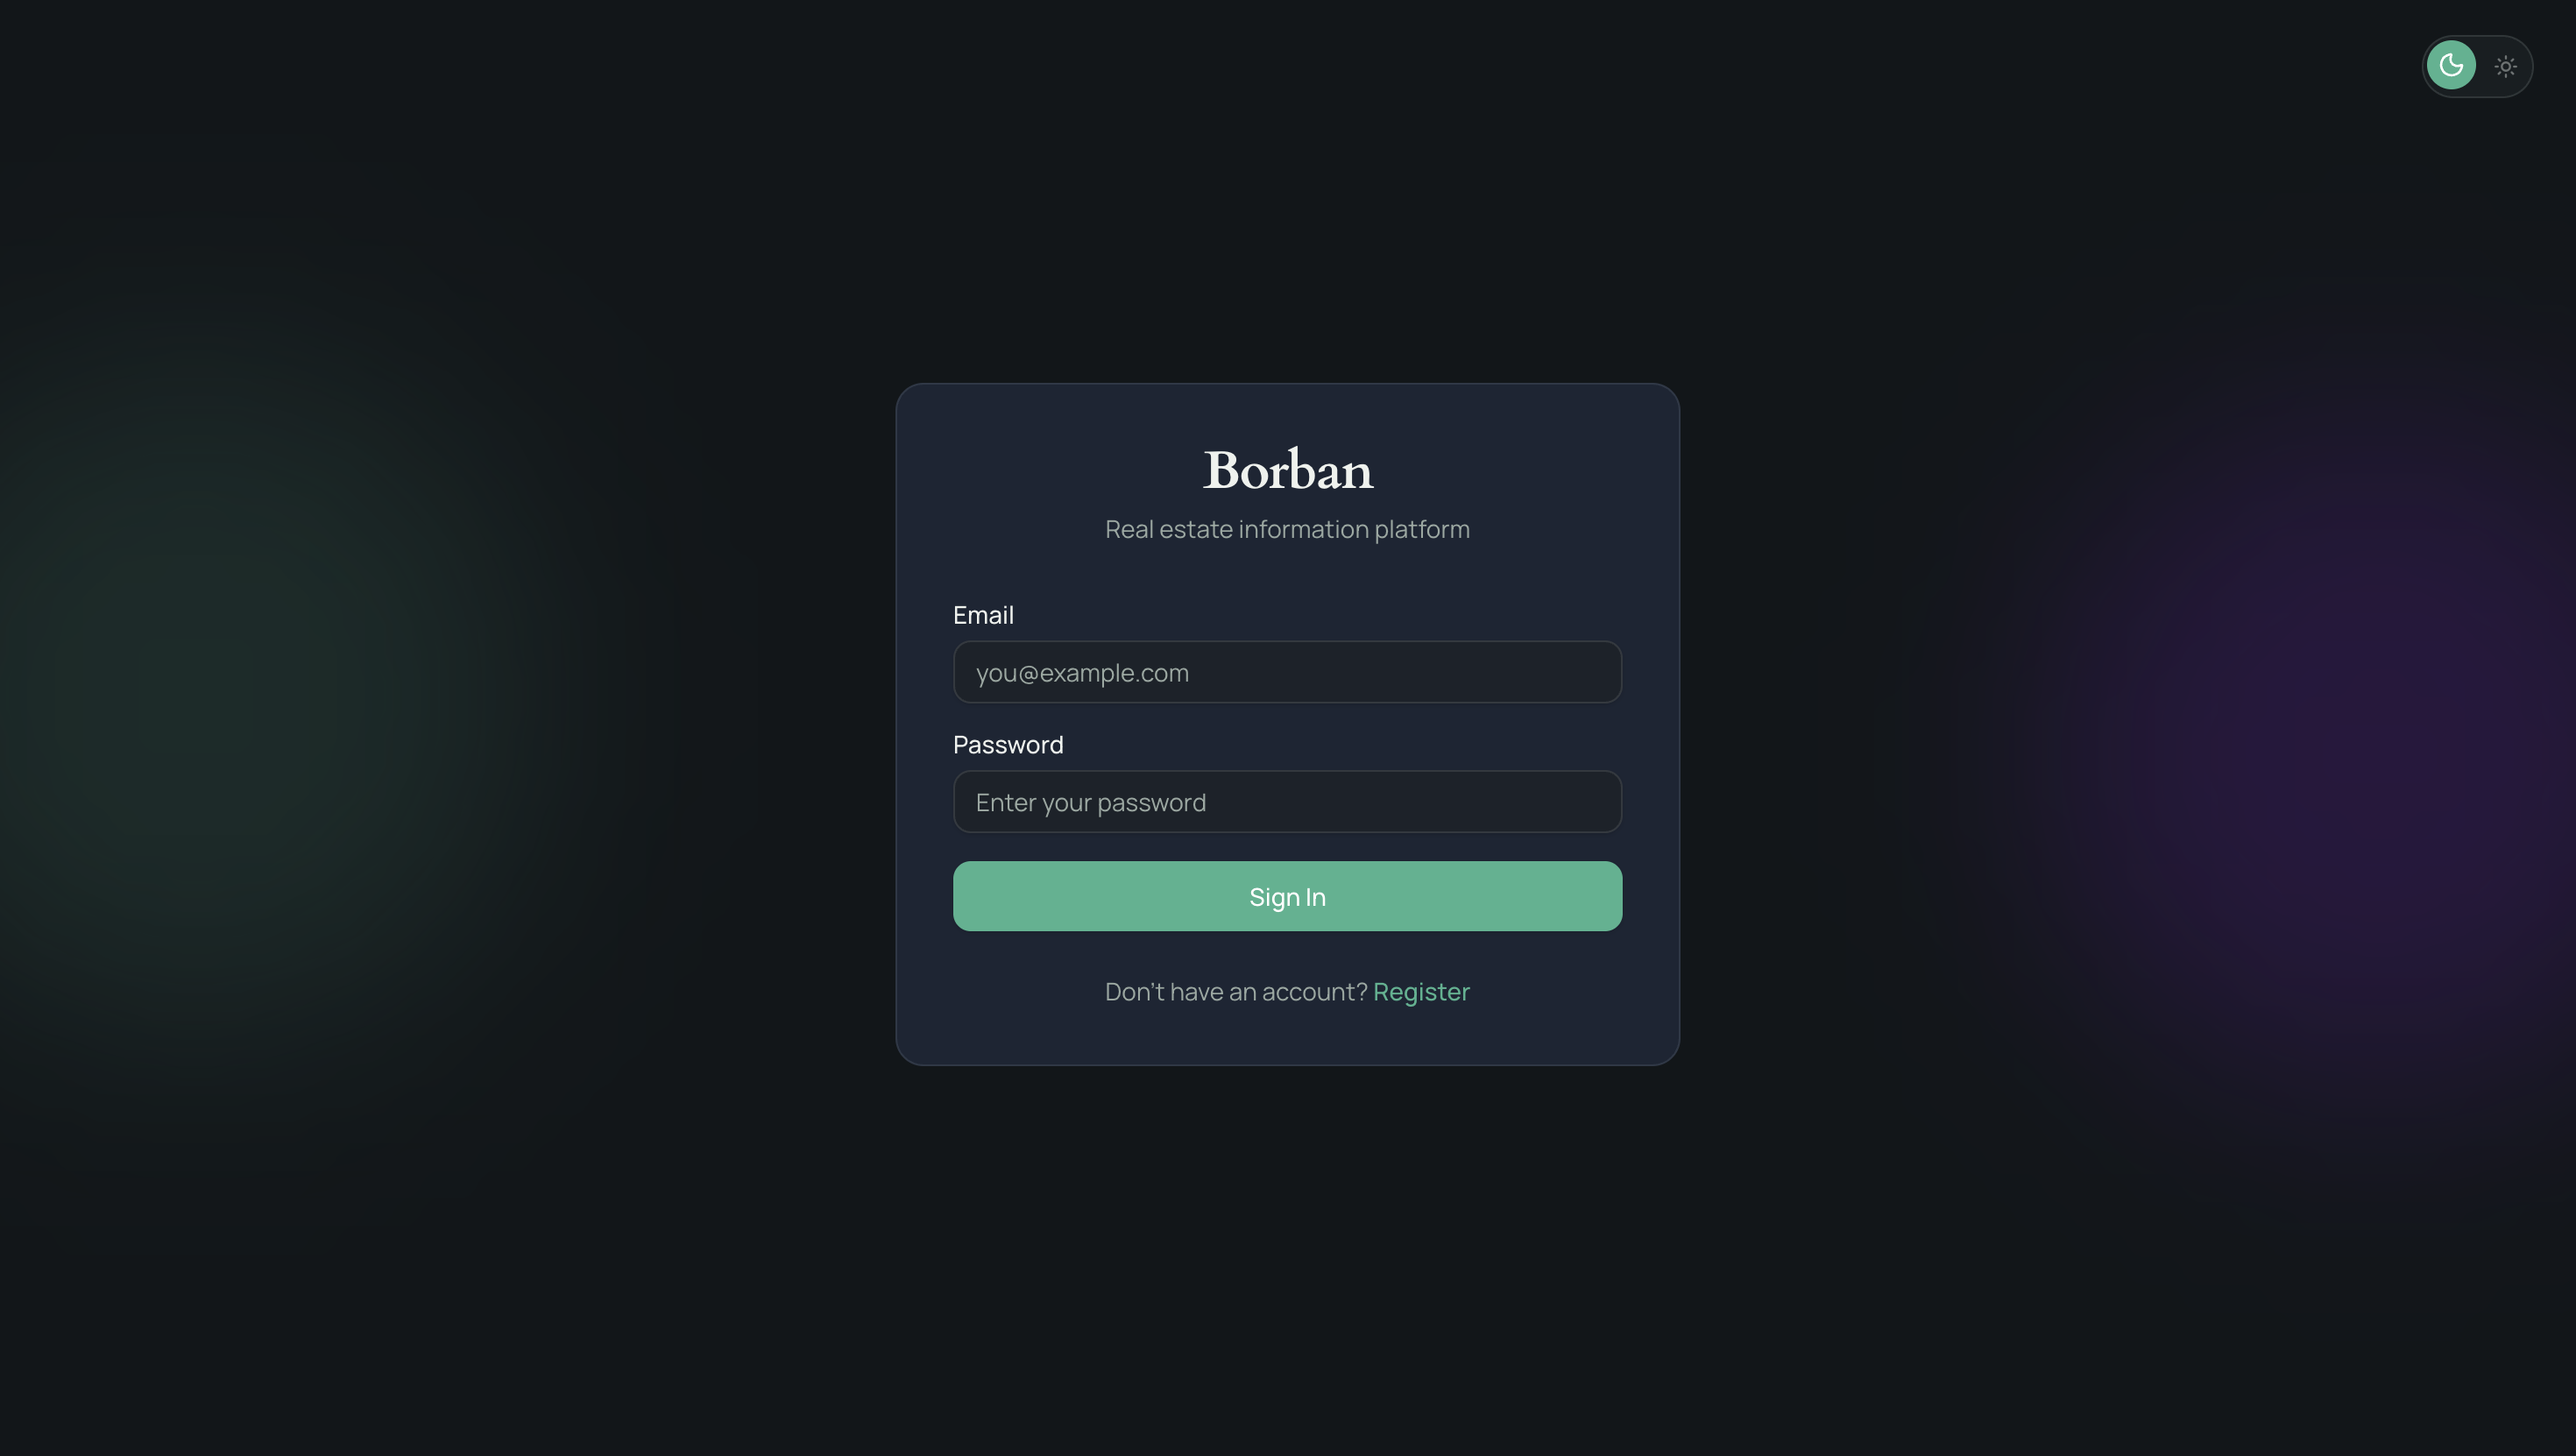
\includegraphics[width=0.96\textwidth]{assets/chapter-7/login-page.png}
    \caption{BorBann Login Page}
    \label{fig:chapter7-login-page}
\end{figure}

\begin{figure}[htbp]
    \centering
    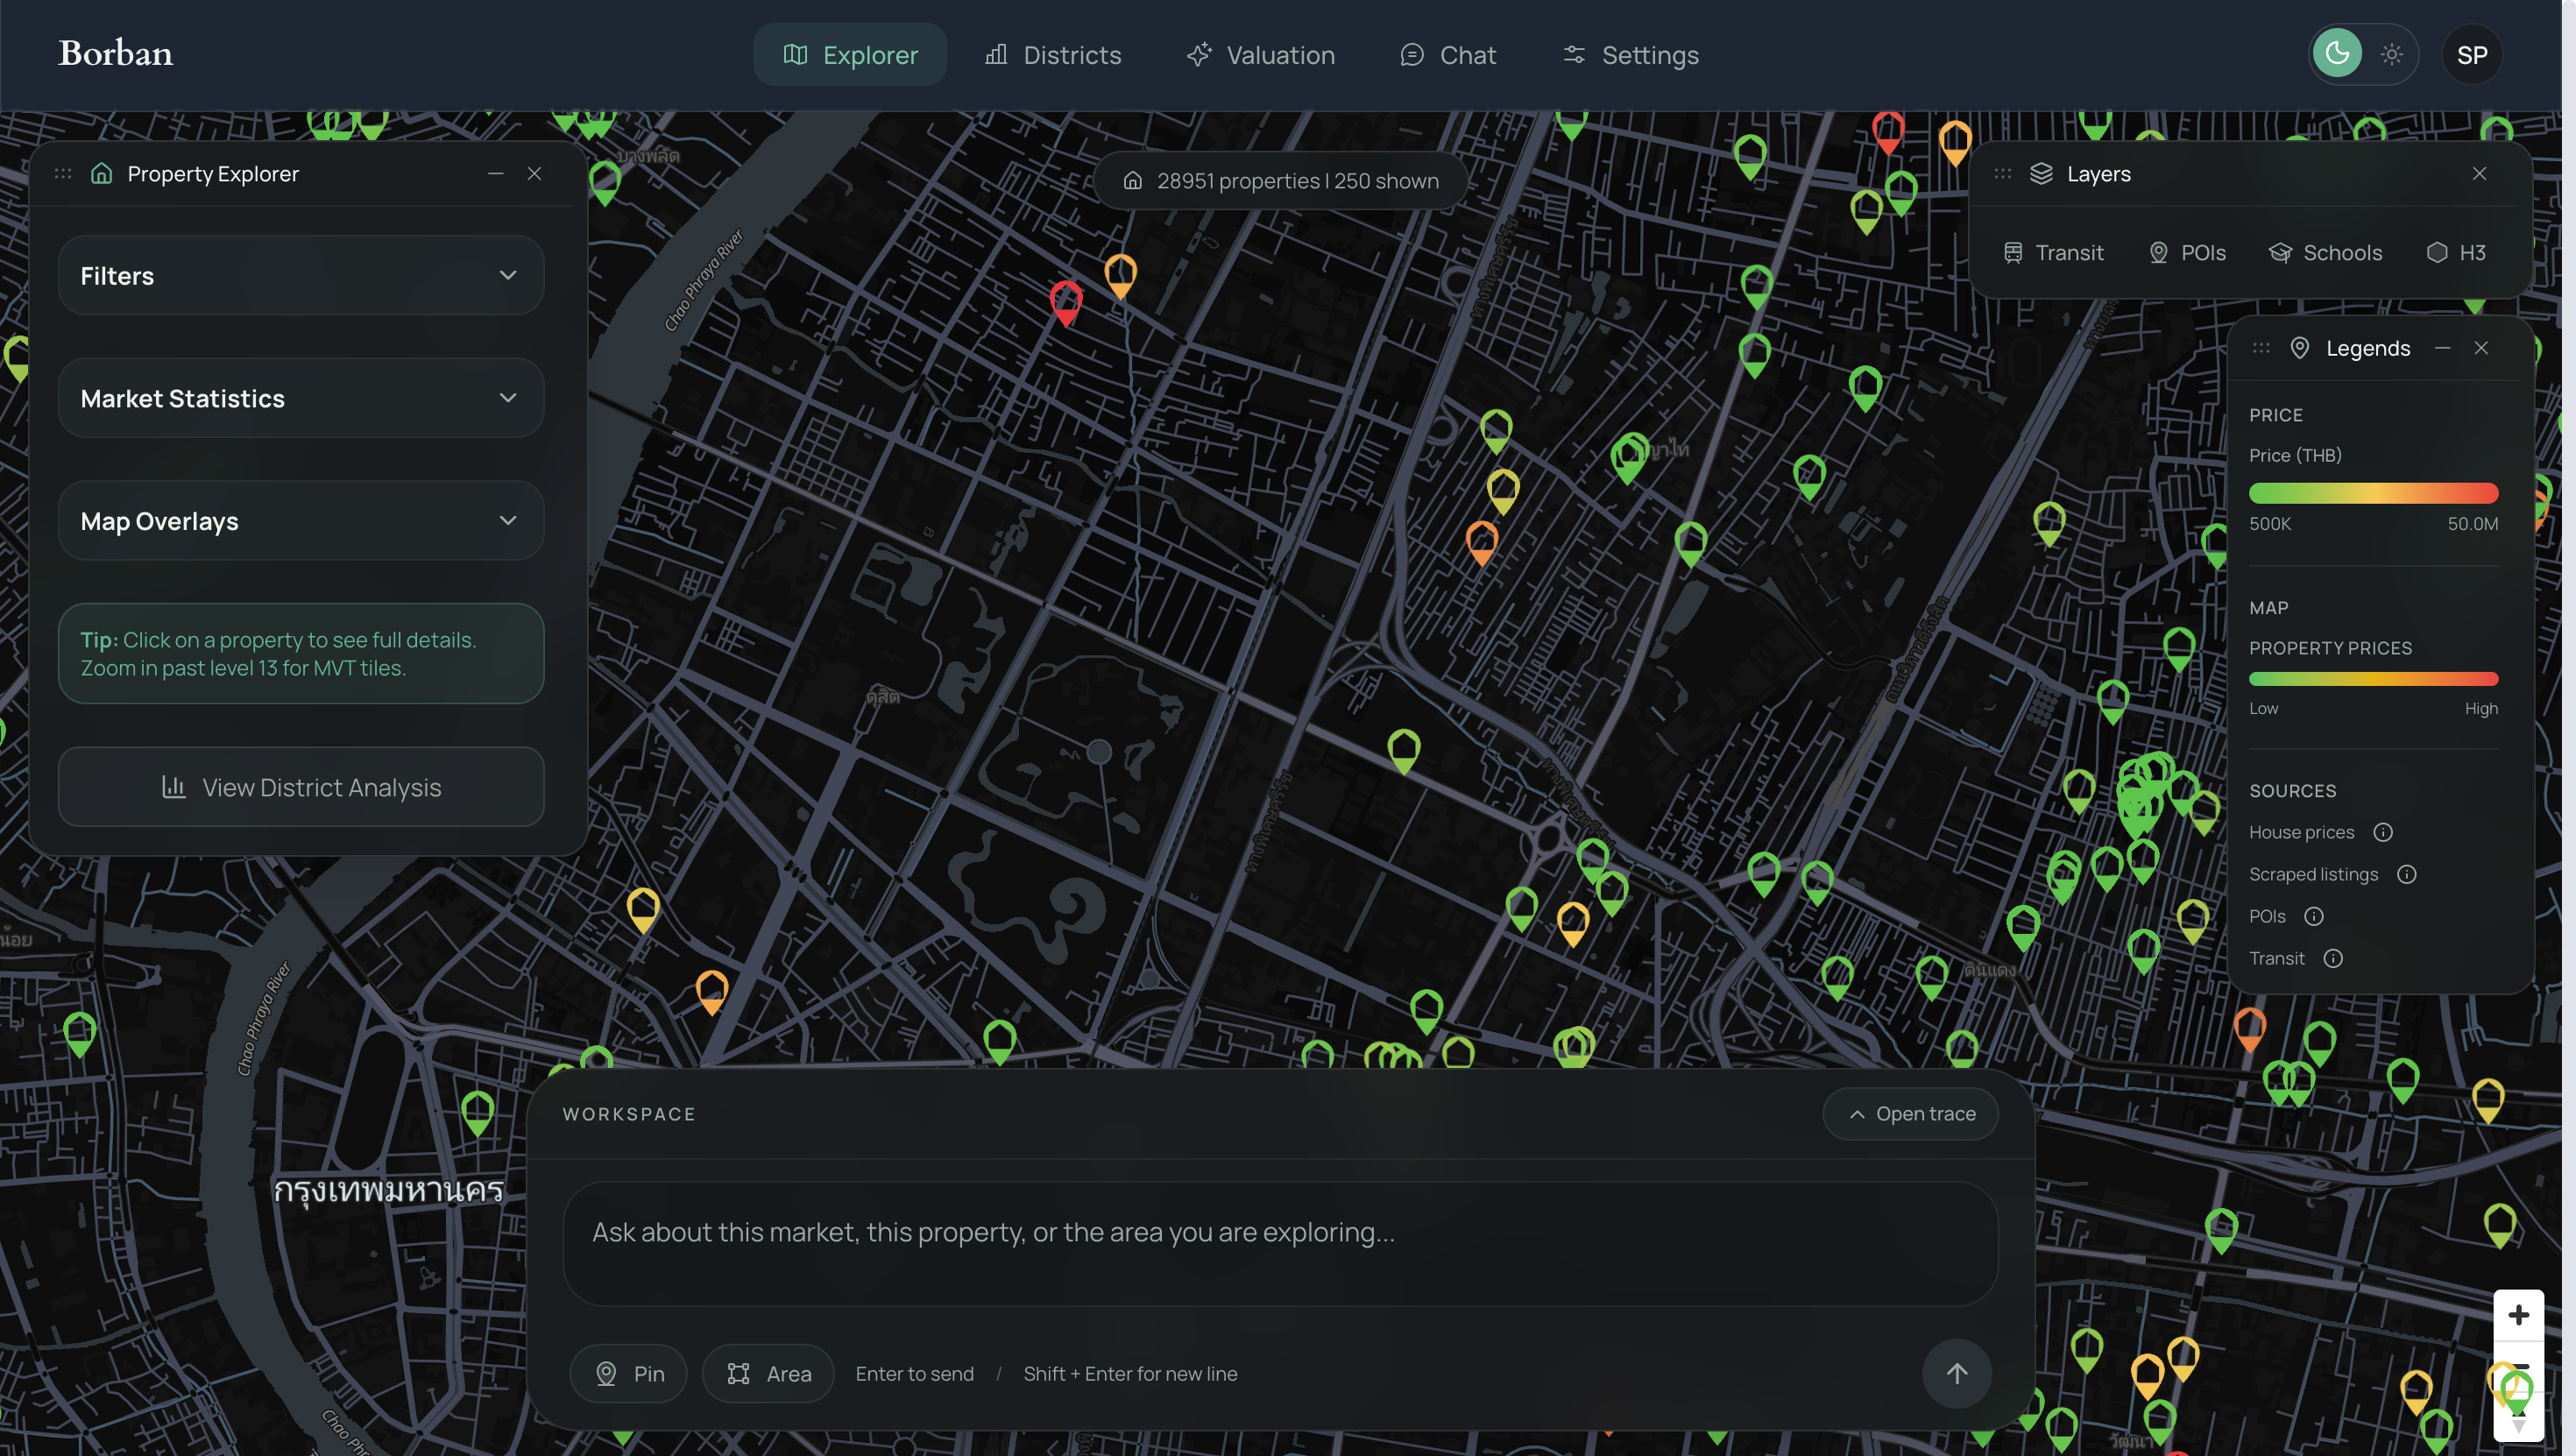
\includegraphics[width=\textwidth]{assets/chapter-7/explorer-page.png}
    \caption{Main Property Explorer Interface}
    \label{fig:chapter7-explorer-page}
\end{figure}

\begin{figure}[htbp]
    \centering
    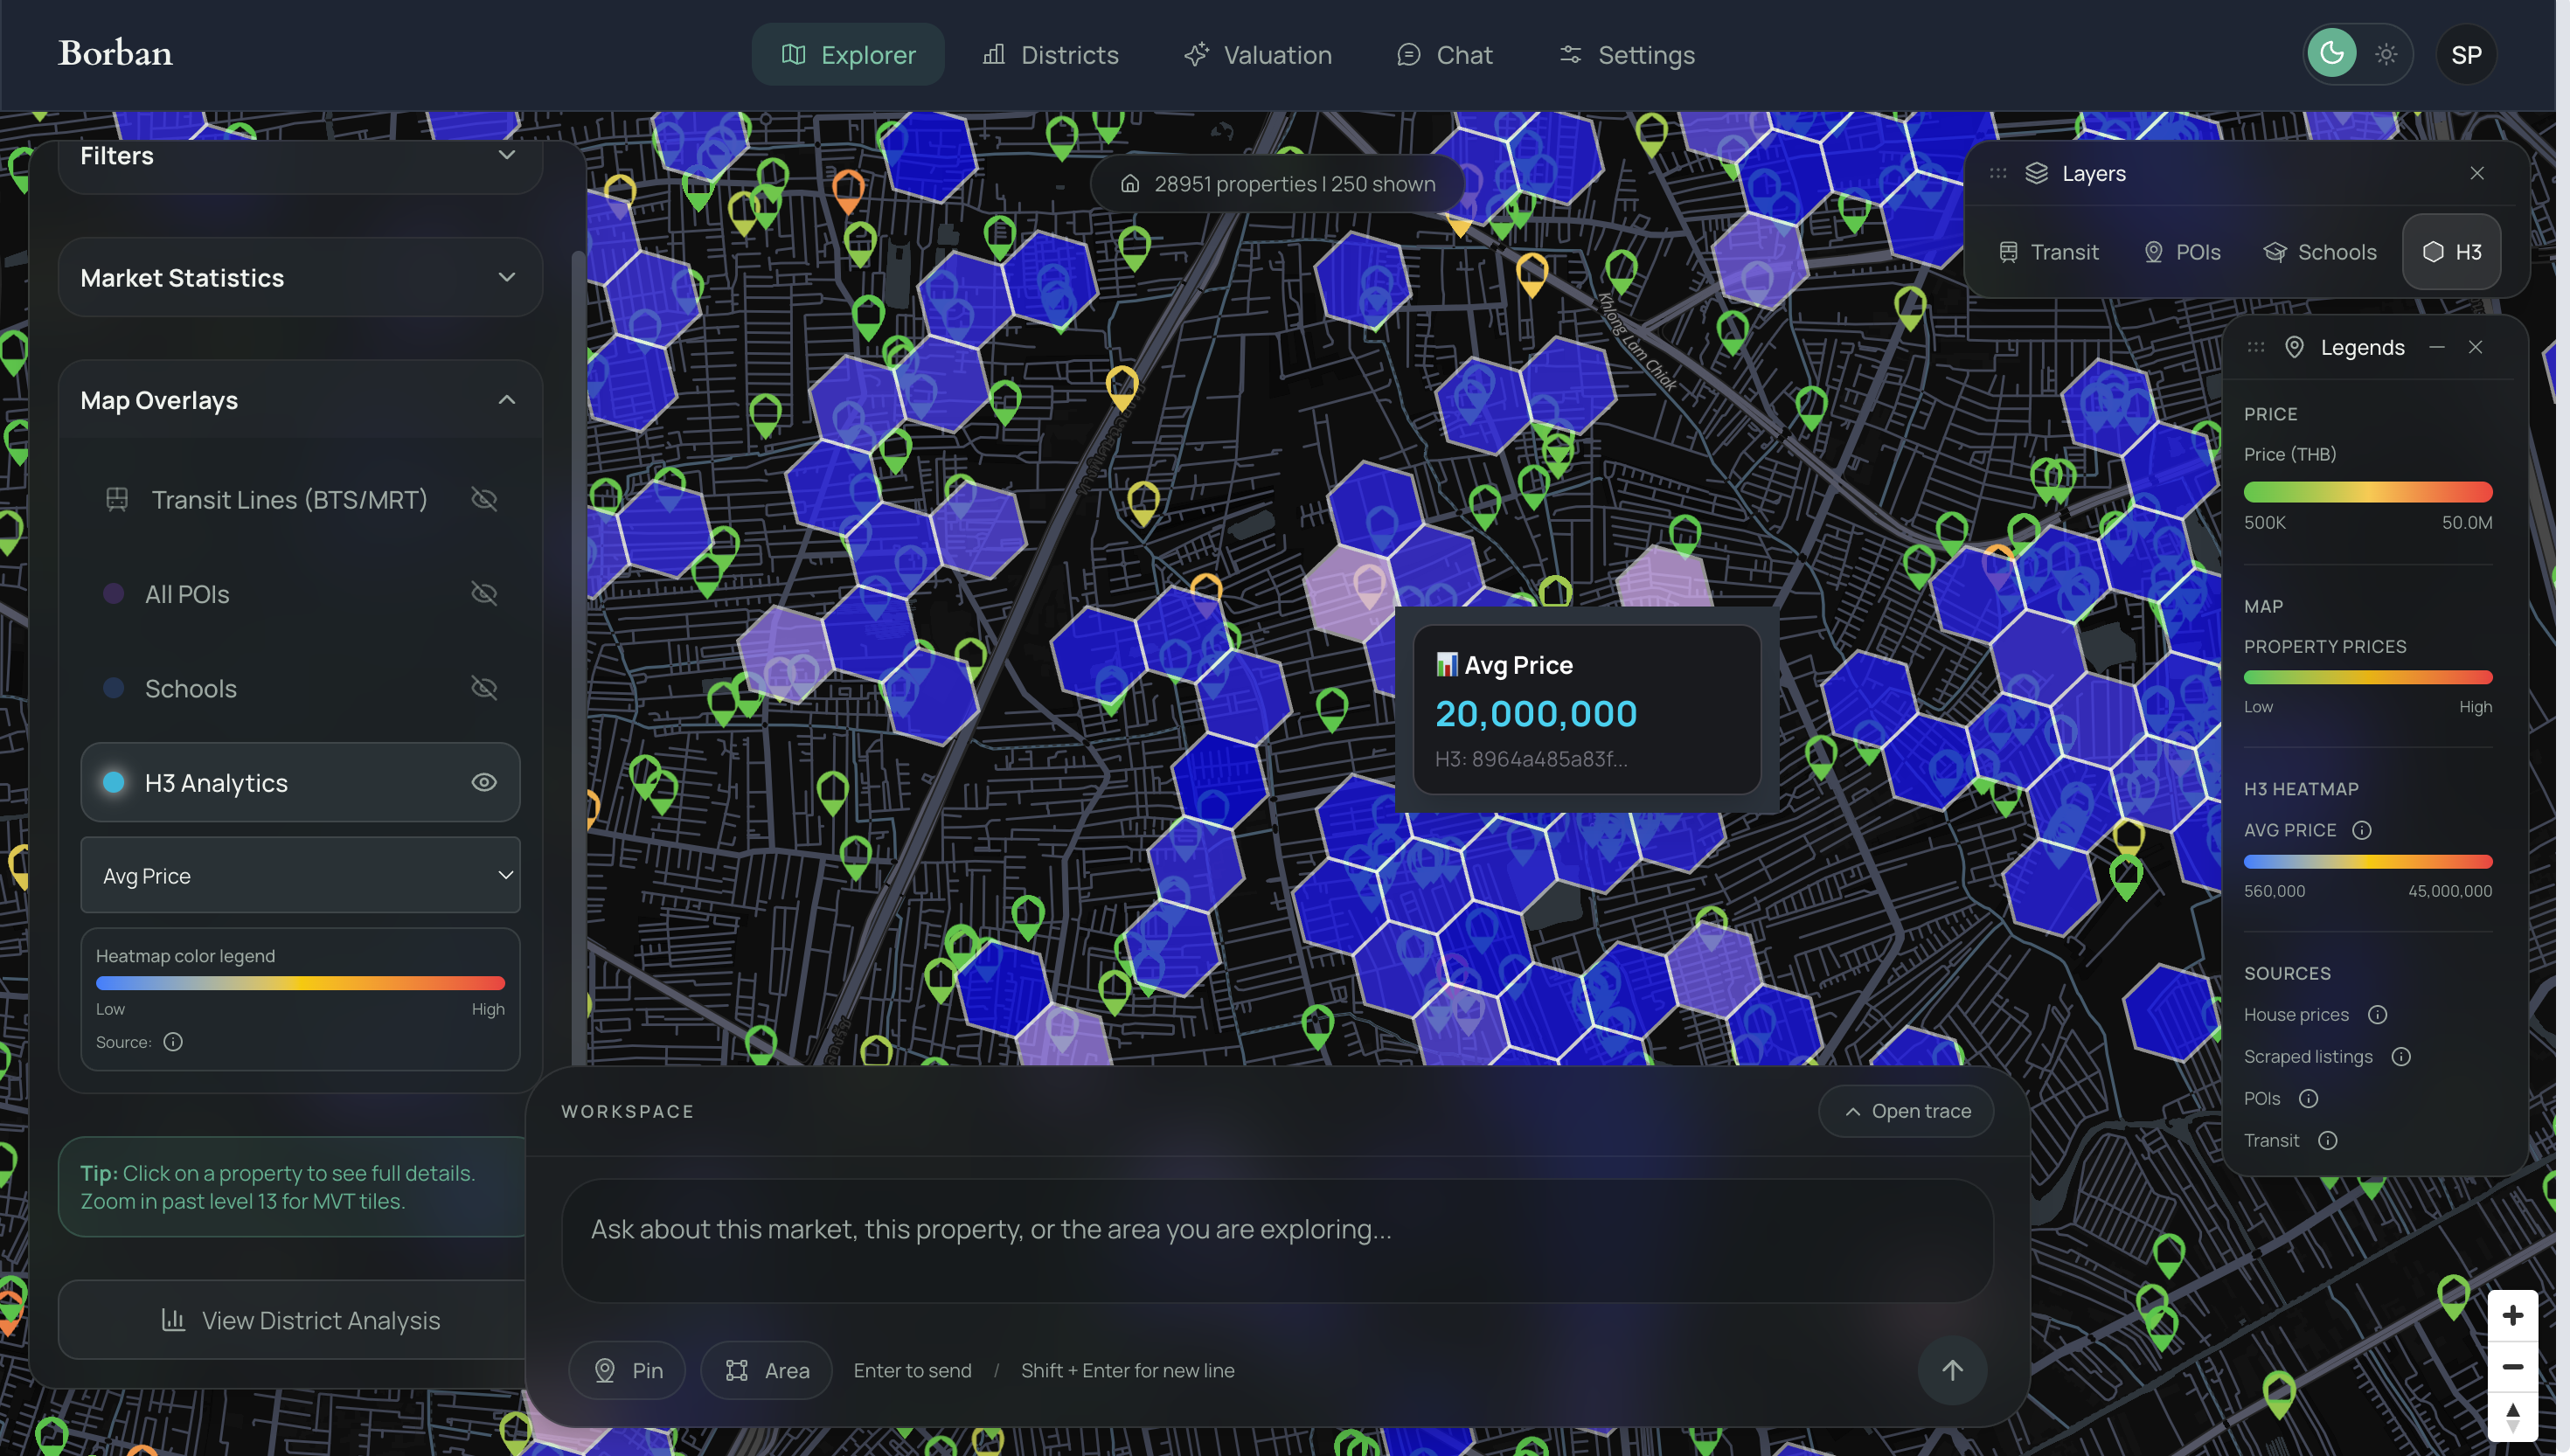
\includegraphics[width=\textwidth]{assets/chapter-7/explorer-page-h3-analytic.png}
    \caption{Explorer Interface with H3 Analytics Layer}
    \label{fig:chapter7-explorer-h3}
\end{figure}

\begin{figure}[htbp]
    \centering
    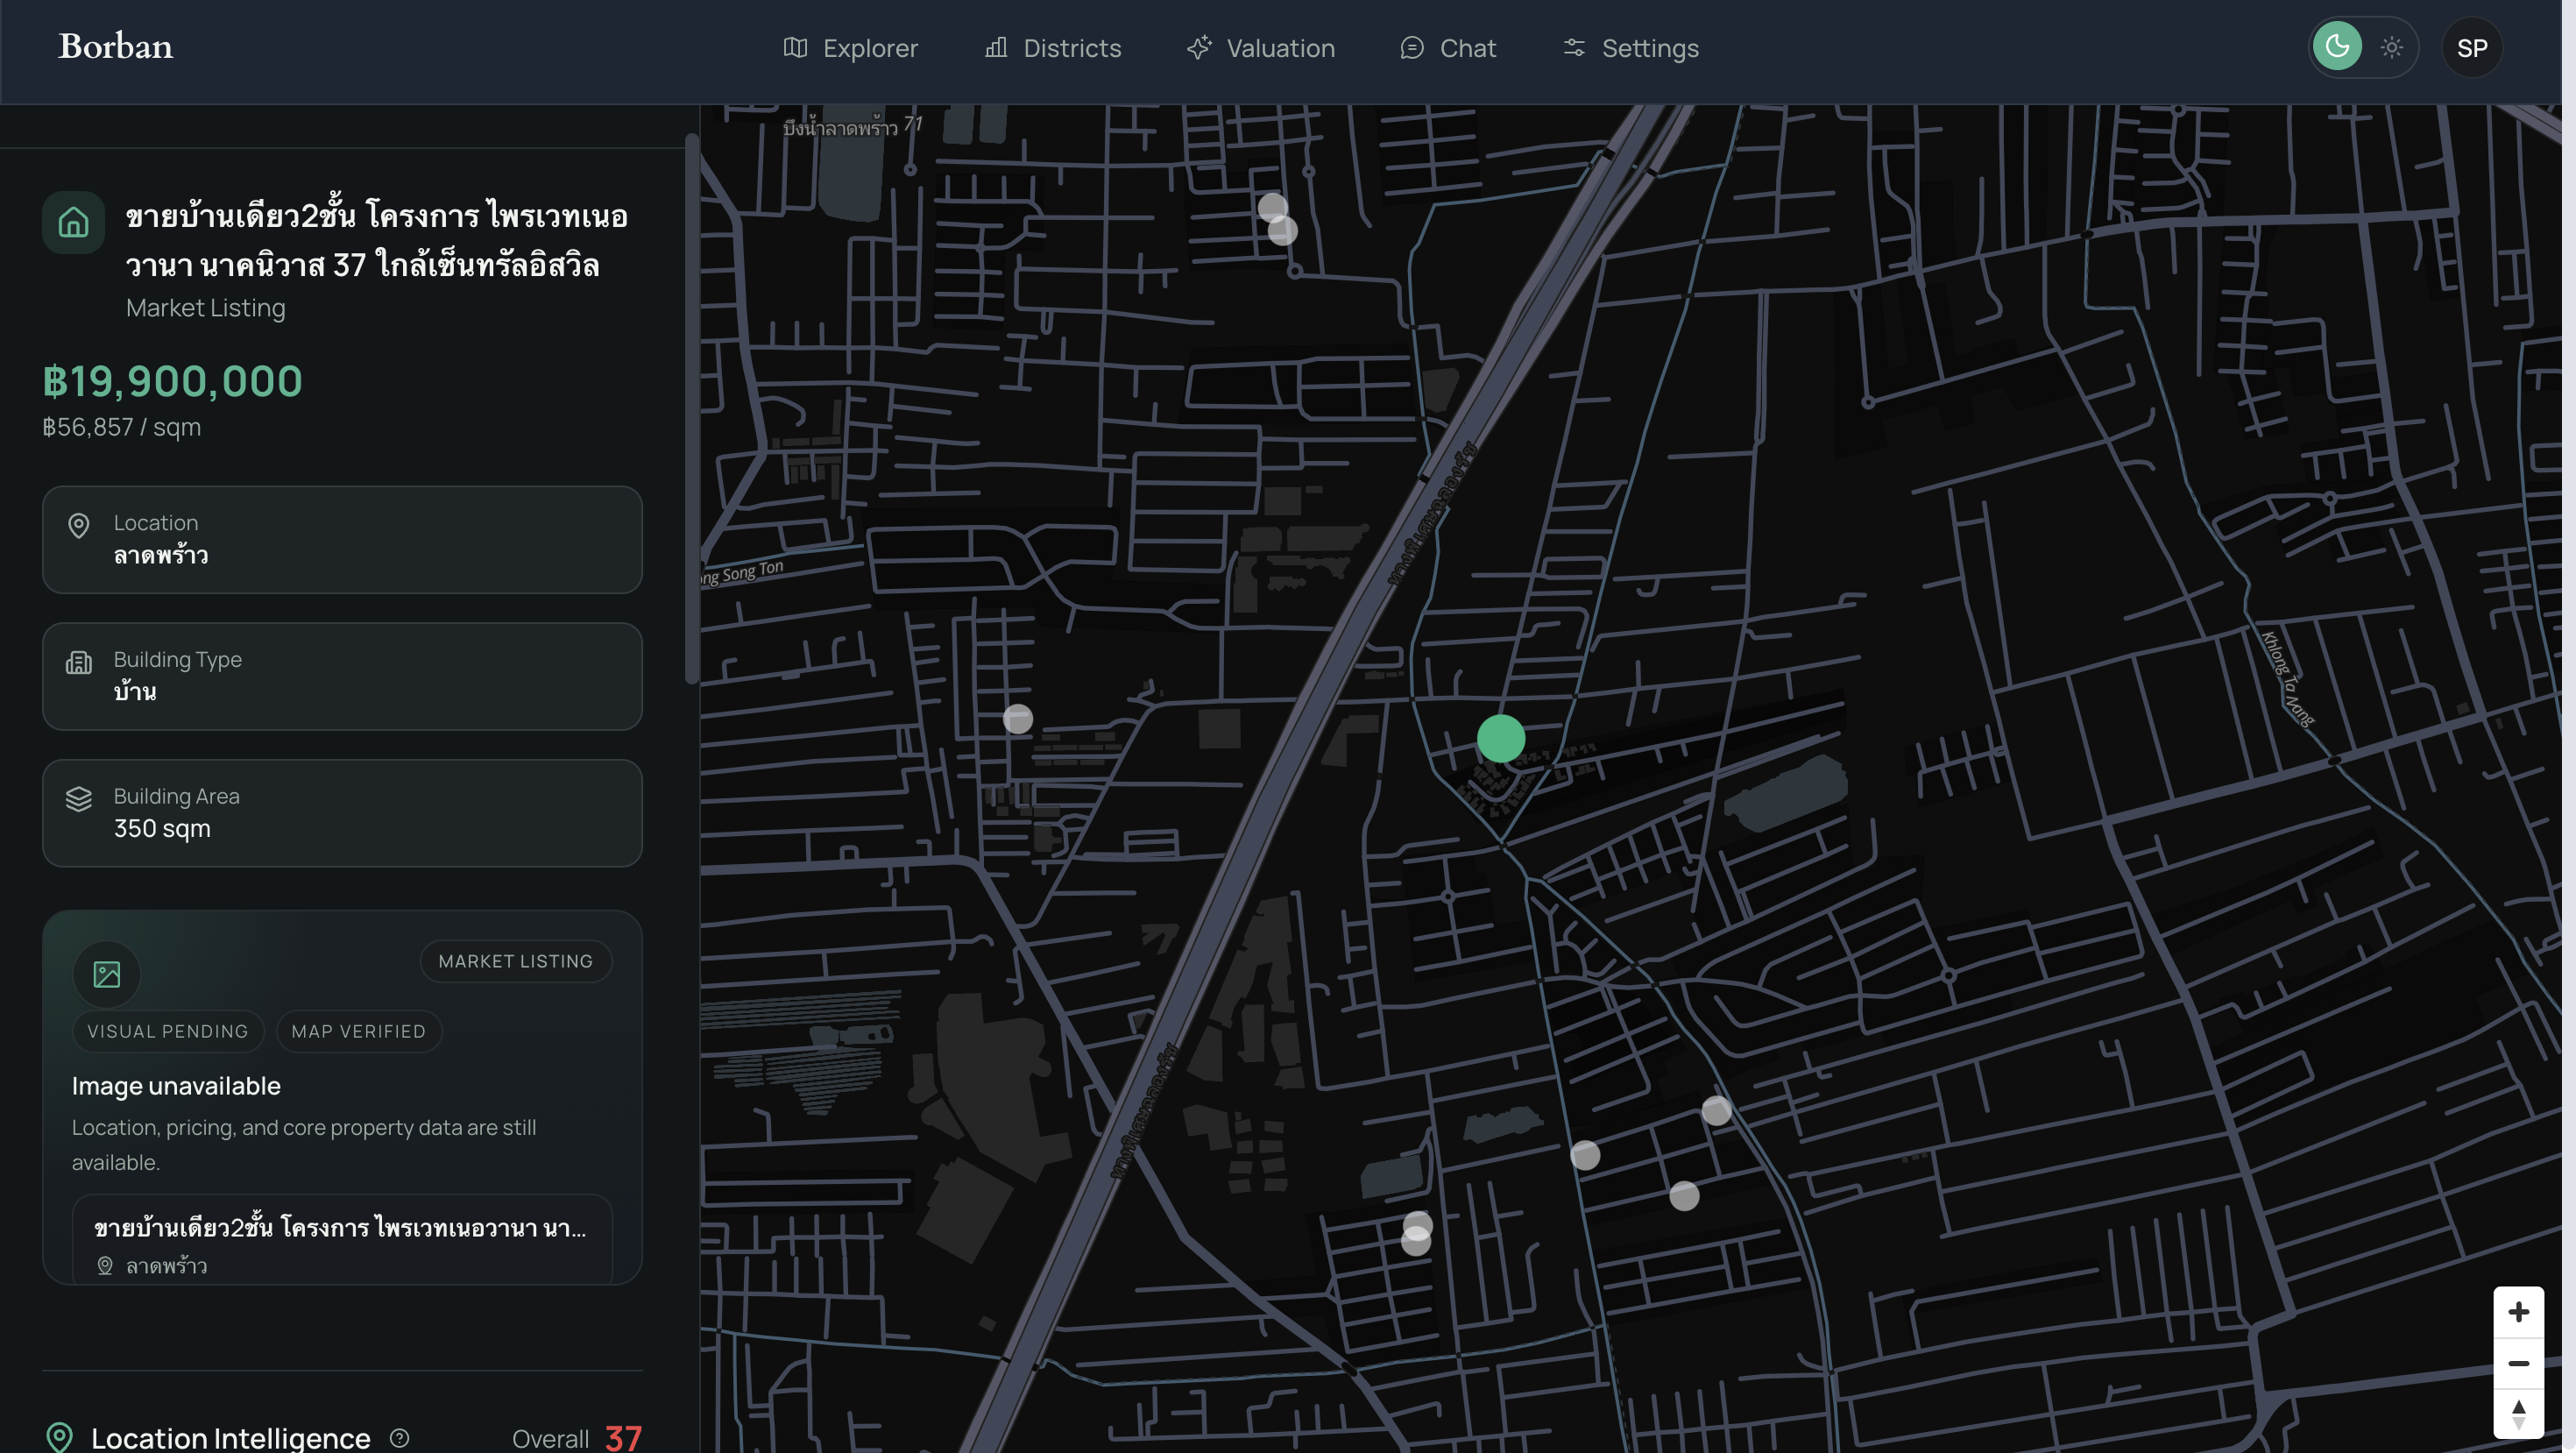
\includegraphics[width=\textwidth]{assets/chapter-7/property-page.png}
    \caption{Property Detail Page}
    \label{fig:chapter7-property-page}
\end{figure}

\begin{figure}[htbp]
    \centering
    \begin{subfigure}[t]{0.48\textwidth}
        \centering
        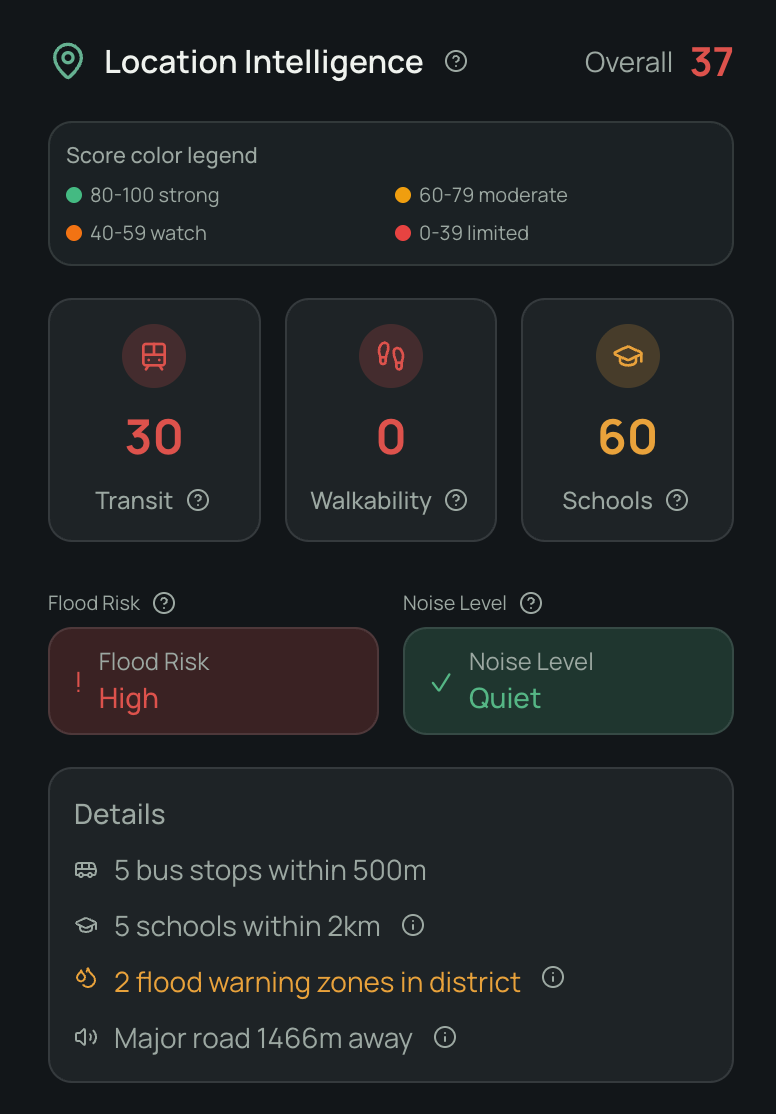
\includegraphics[width=0.78\textwidth]{assets/chapter-7/property-page-location-intelligence.png}
        \caption{Location intelligence panel}
    \end{subfigure}
    \hfill
    \begin{subfigure}[t]{0.48\textwidth}
        \centering
        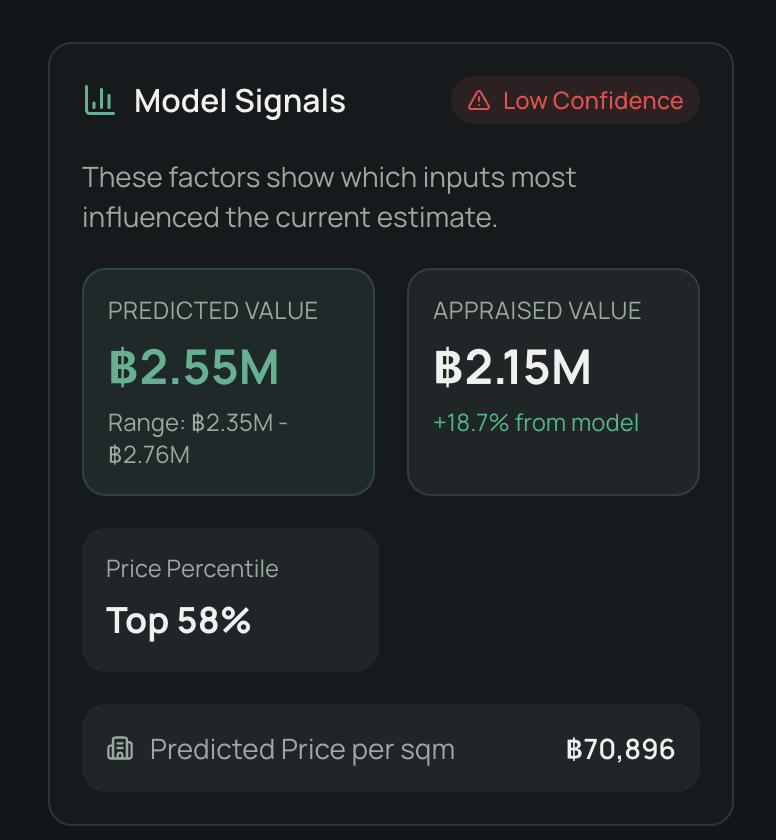
\includegraphics[width=0.78\textwidth]{assets/chapter-7/property-page-model-signal.png}
        \caption{Model signal summary}
    \end{subfigure}
    \caption{Property-Level Analytical Panels}
    \label{fig:chapter7-property-panels}
\end{figure}

\begin{figure}[htbp]
    \centering
    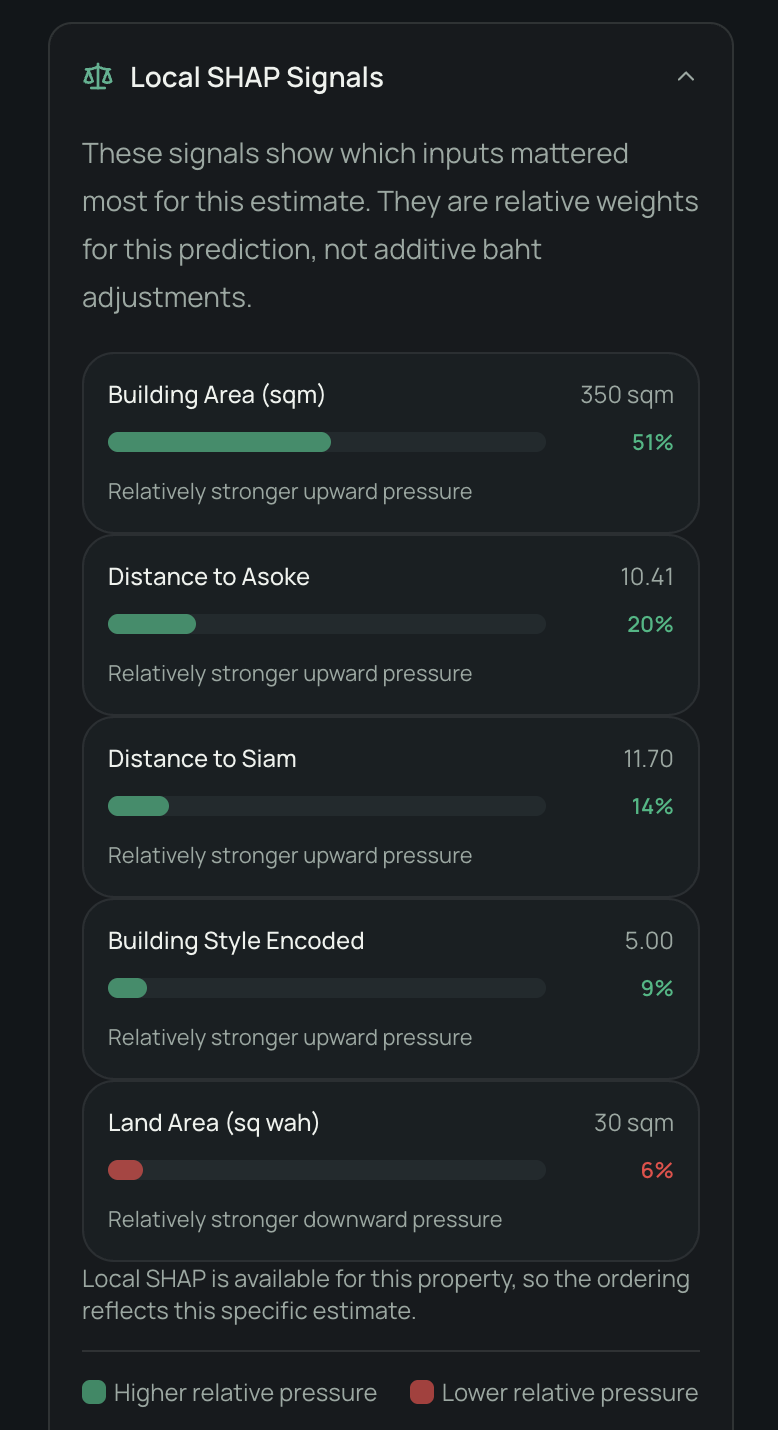
\includegraphics[width=0.34\textwidth]{assets/chapter-7/property-page-local-shap.png}
    \caption{Property Page Local SHAP Explanation}
    \label{fig:chapter7-property-shap}
\end{figure}

\begin{figure}[htbp]
    \centering
    \begin{subfigure}[t]{0.49\textwidth}
        \centering
        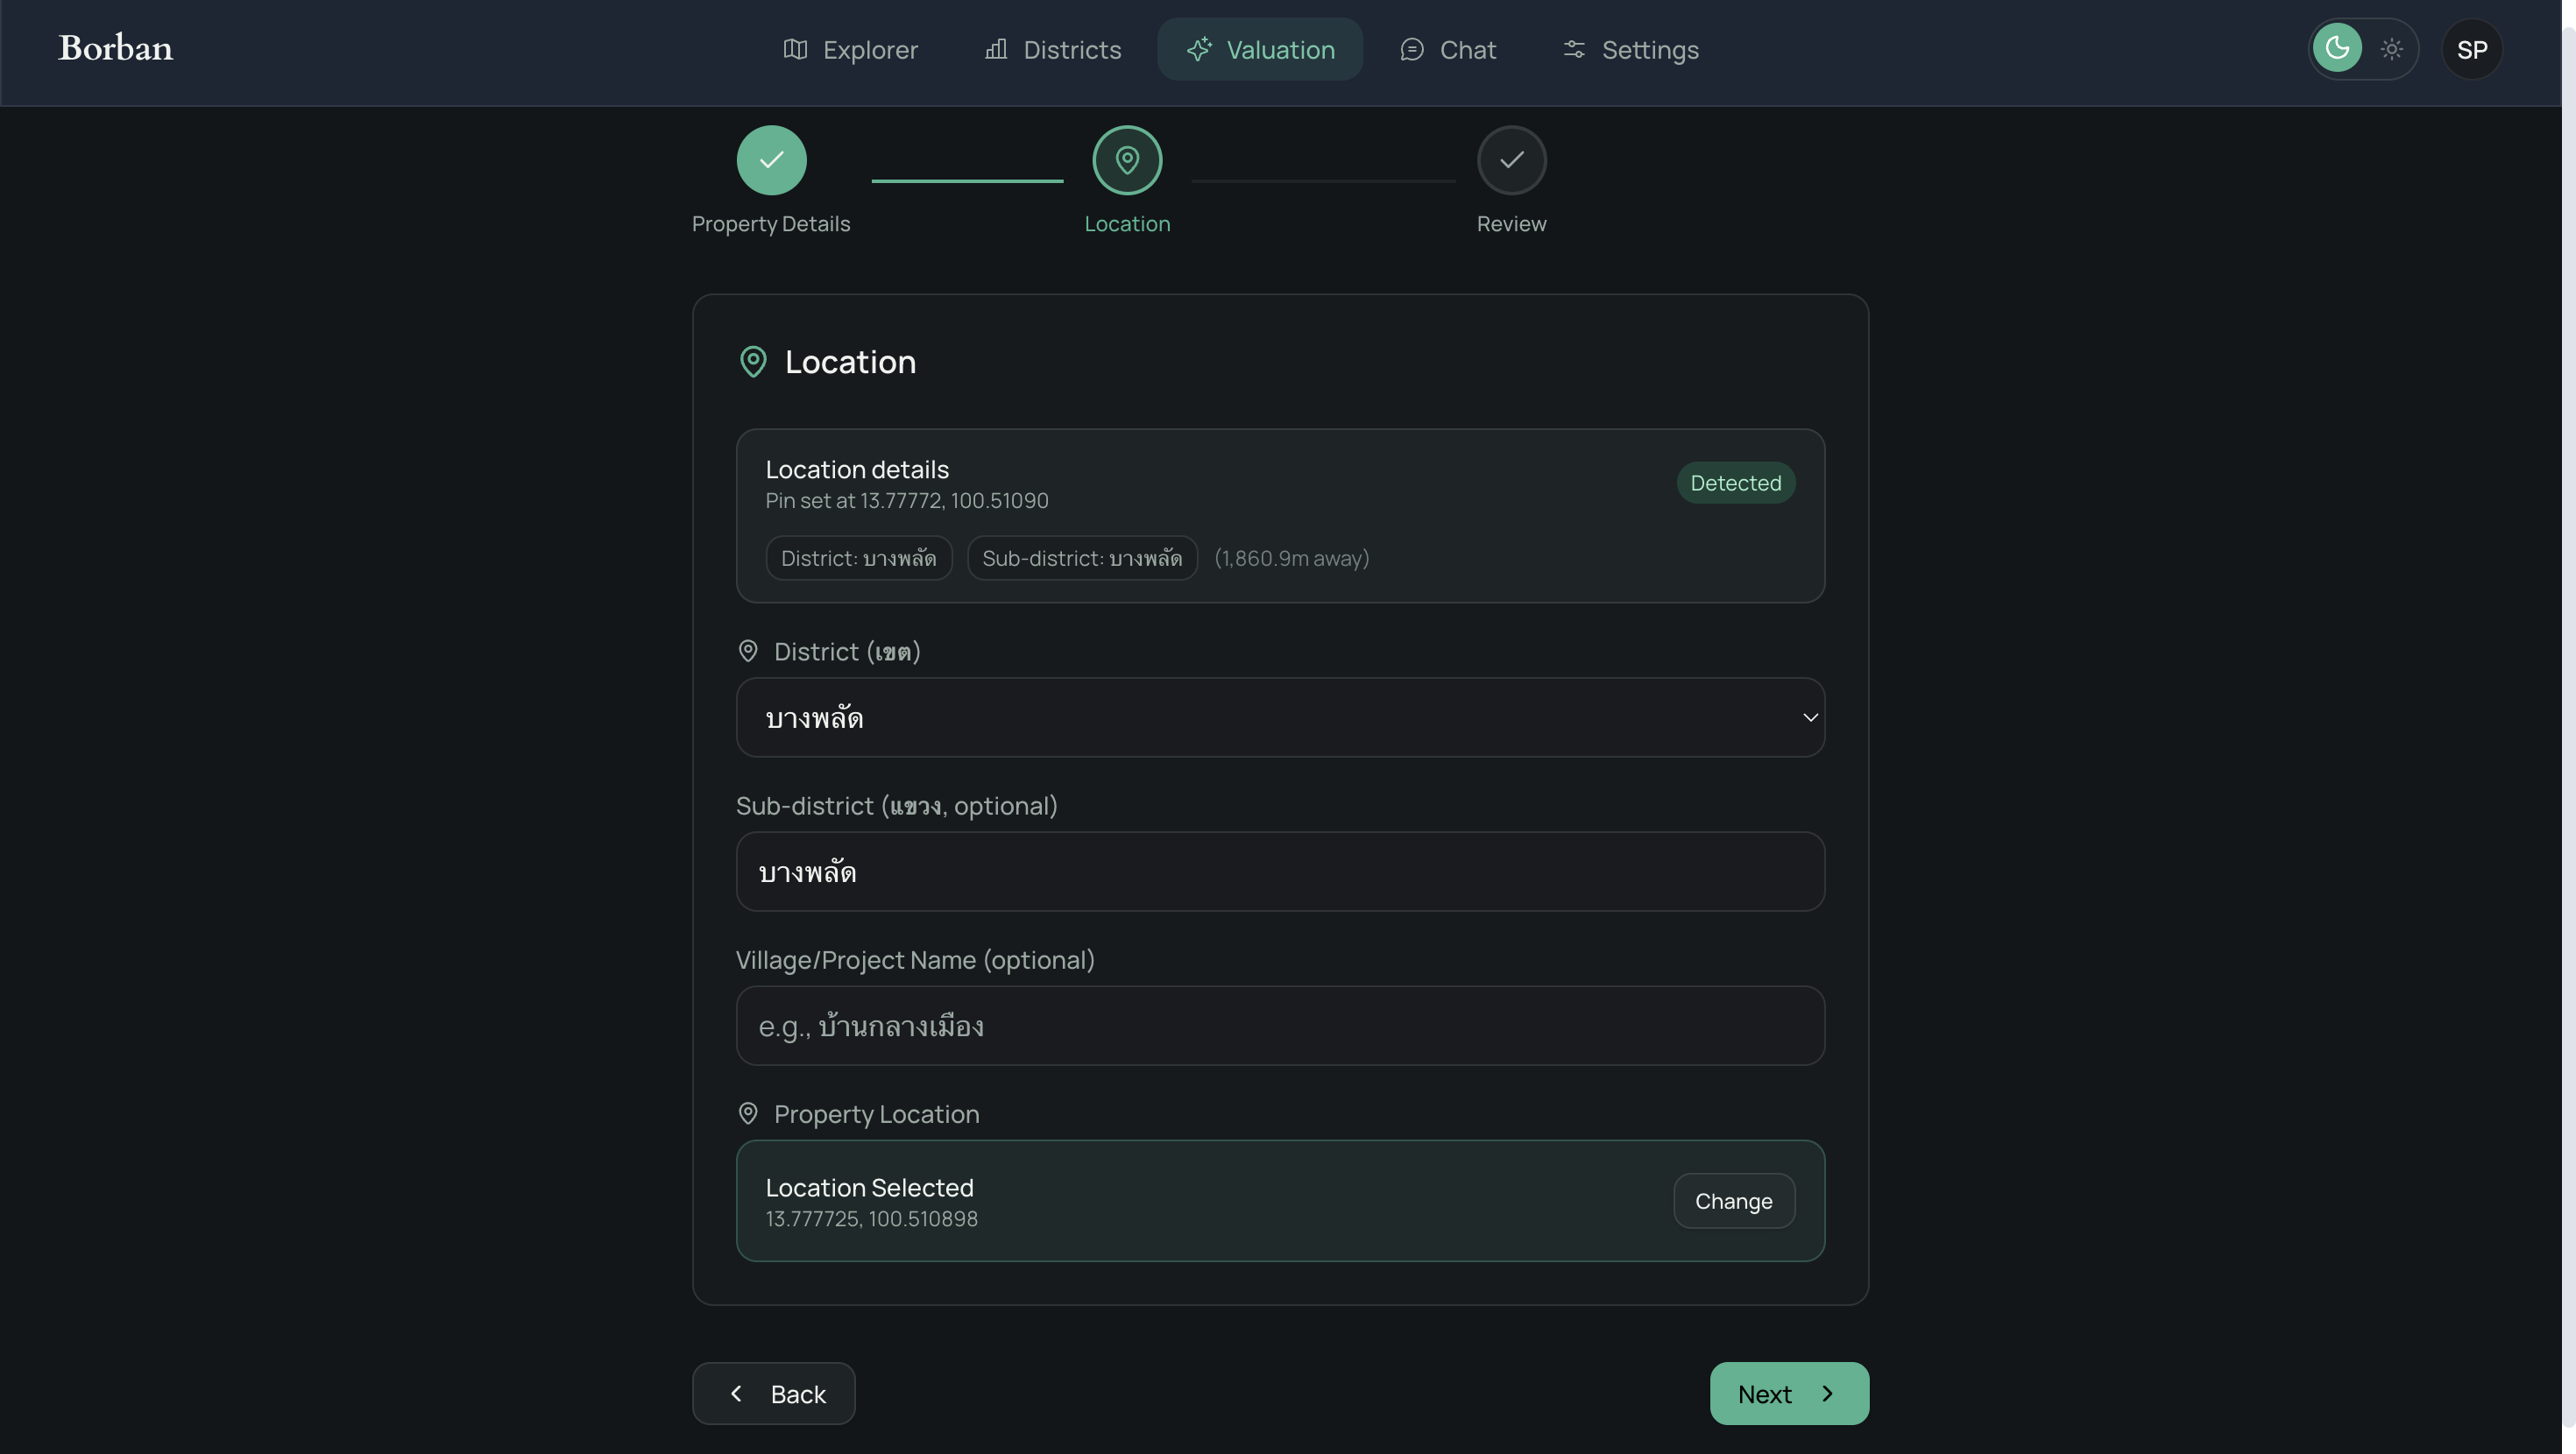
\includegraphics[width=\textwidth]{assets/chapter-7/property-valuation-page-input.png}
        \caption{Valuation request form}
    \end{subfigure}
    \hfill
    \begin{subfigure}[t]{0.49\textwidth}
        \centering
        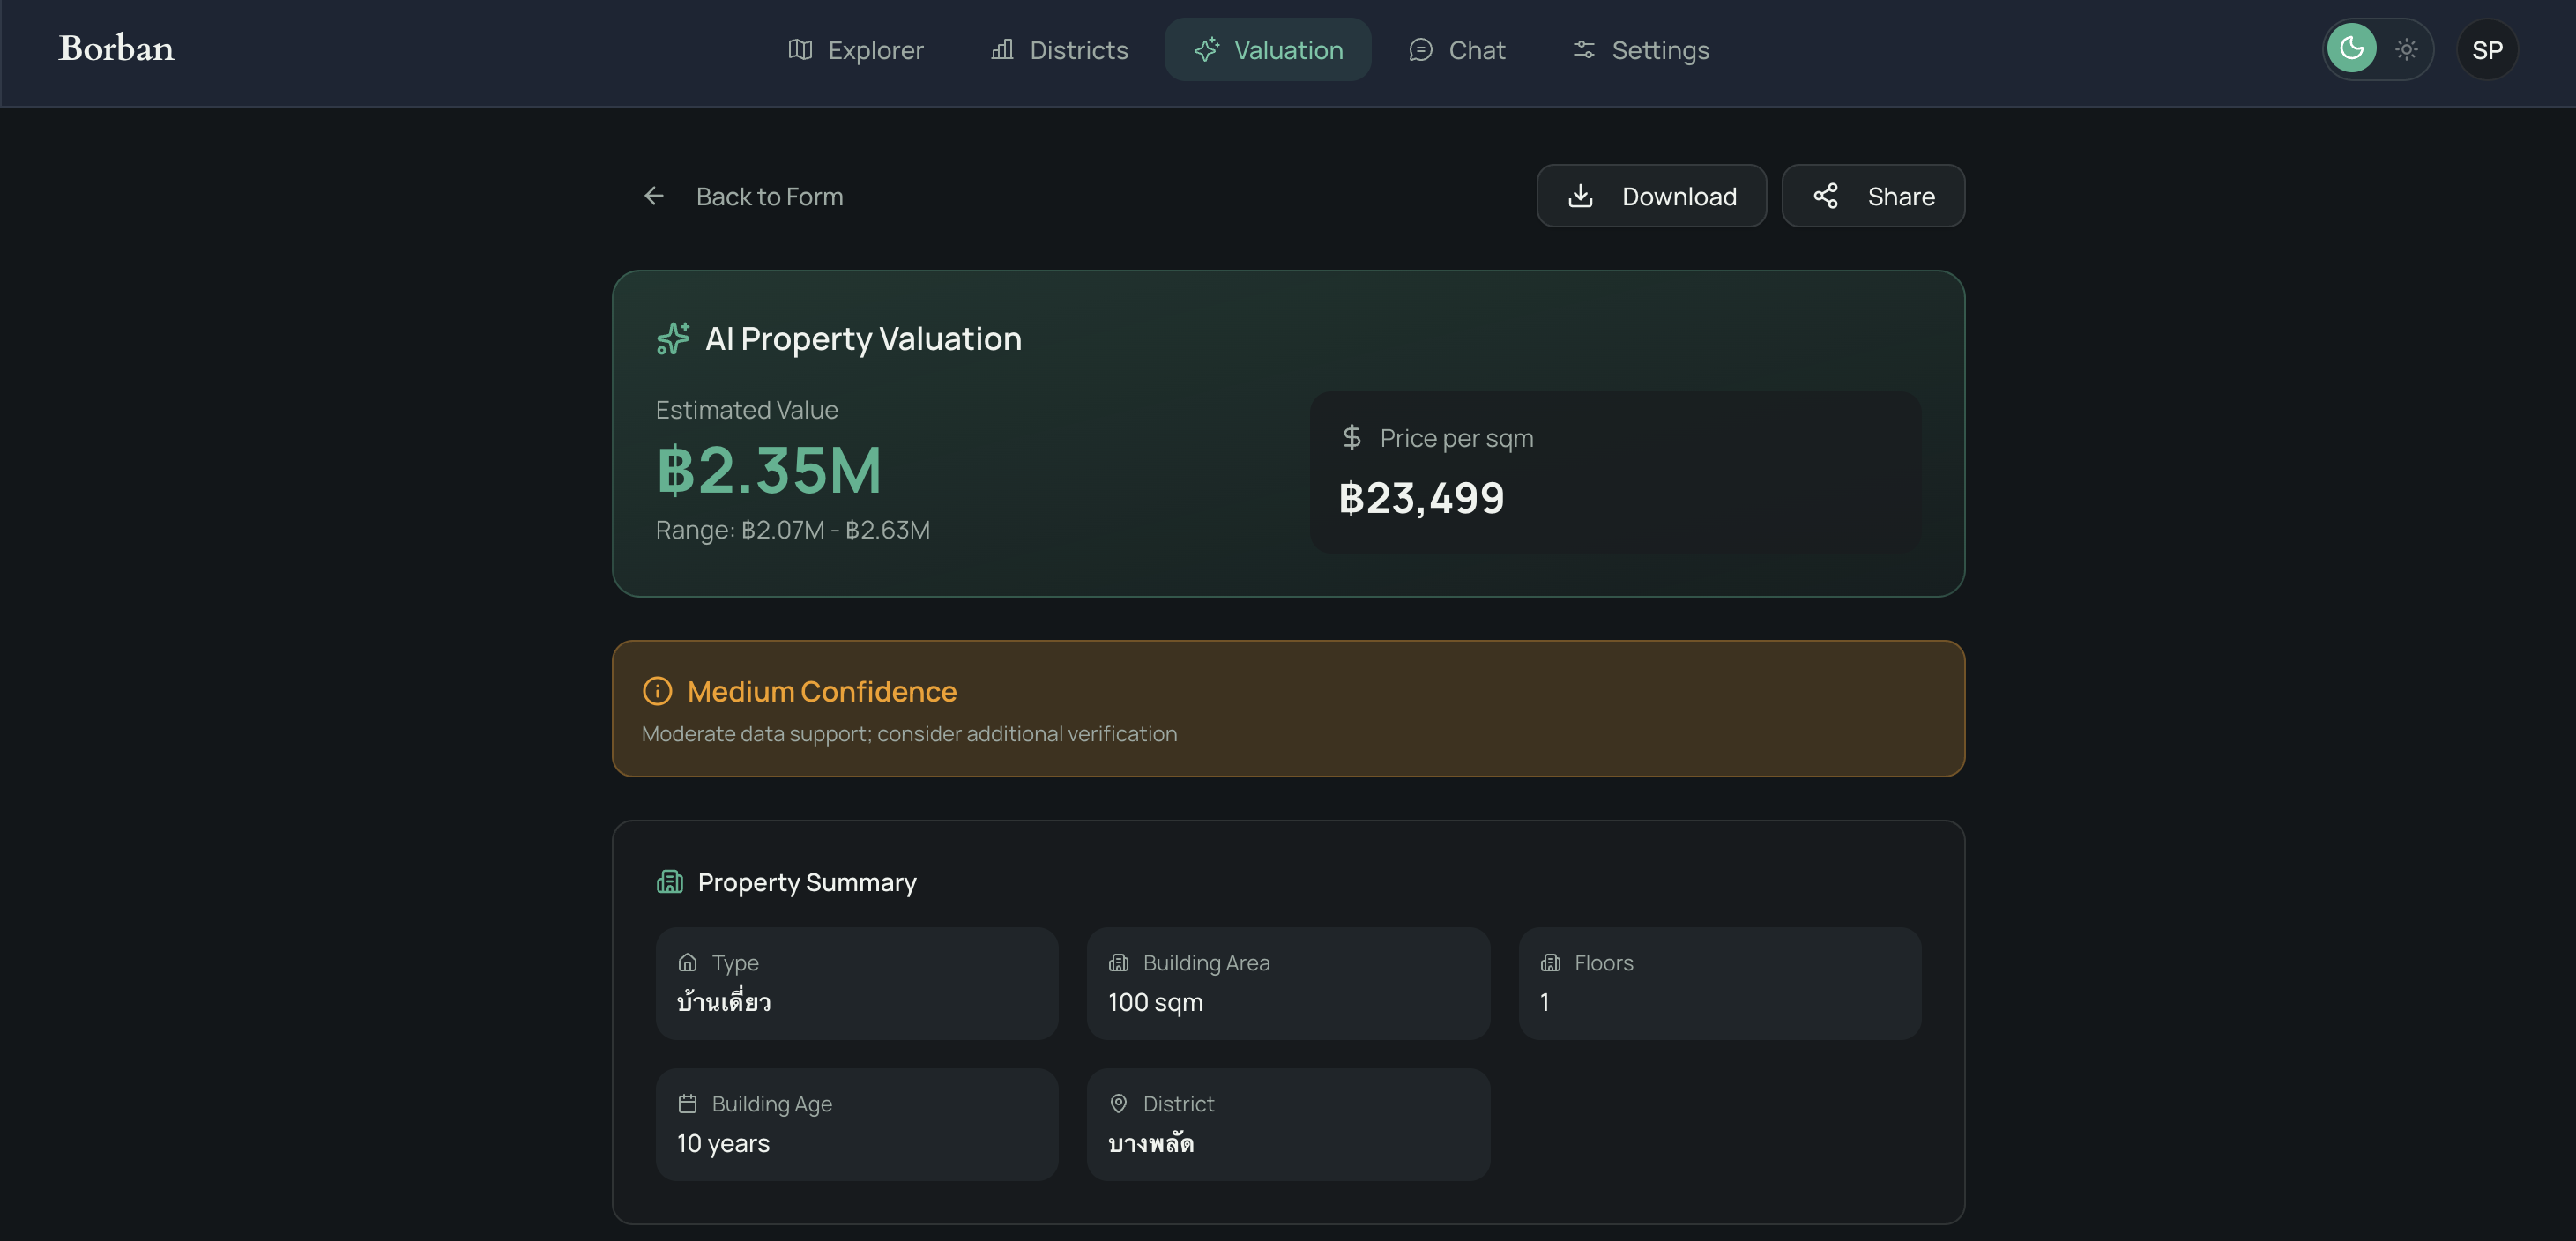
\includegraphics[width=\textwidth]{assets/chapter-7/property-valuation-page.png}
        \caption{Valuation report page}
    \end{subfigure}
    \caption{Valuation Workflow Interfaces}
    \label{fig:chapter7-valuation-pages}
\end{figure}

\begin{figure}[htbp]
    \centering
    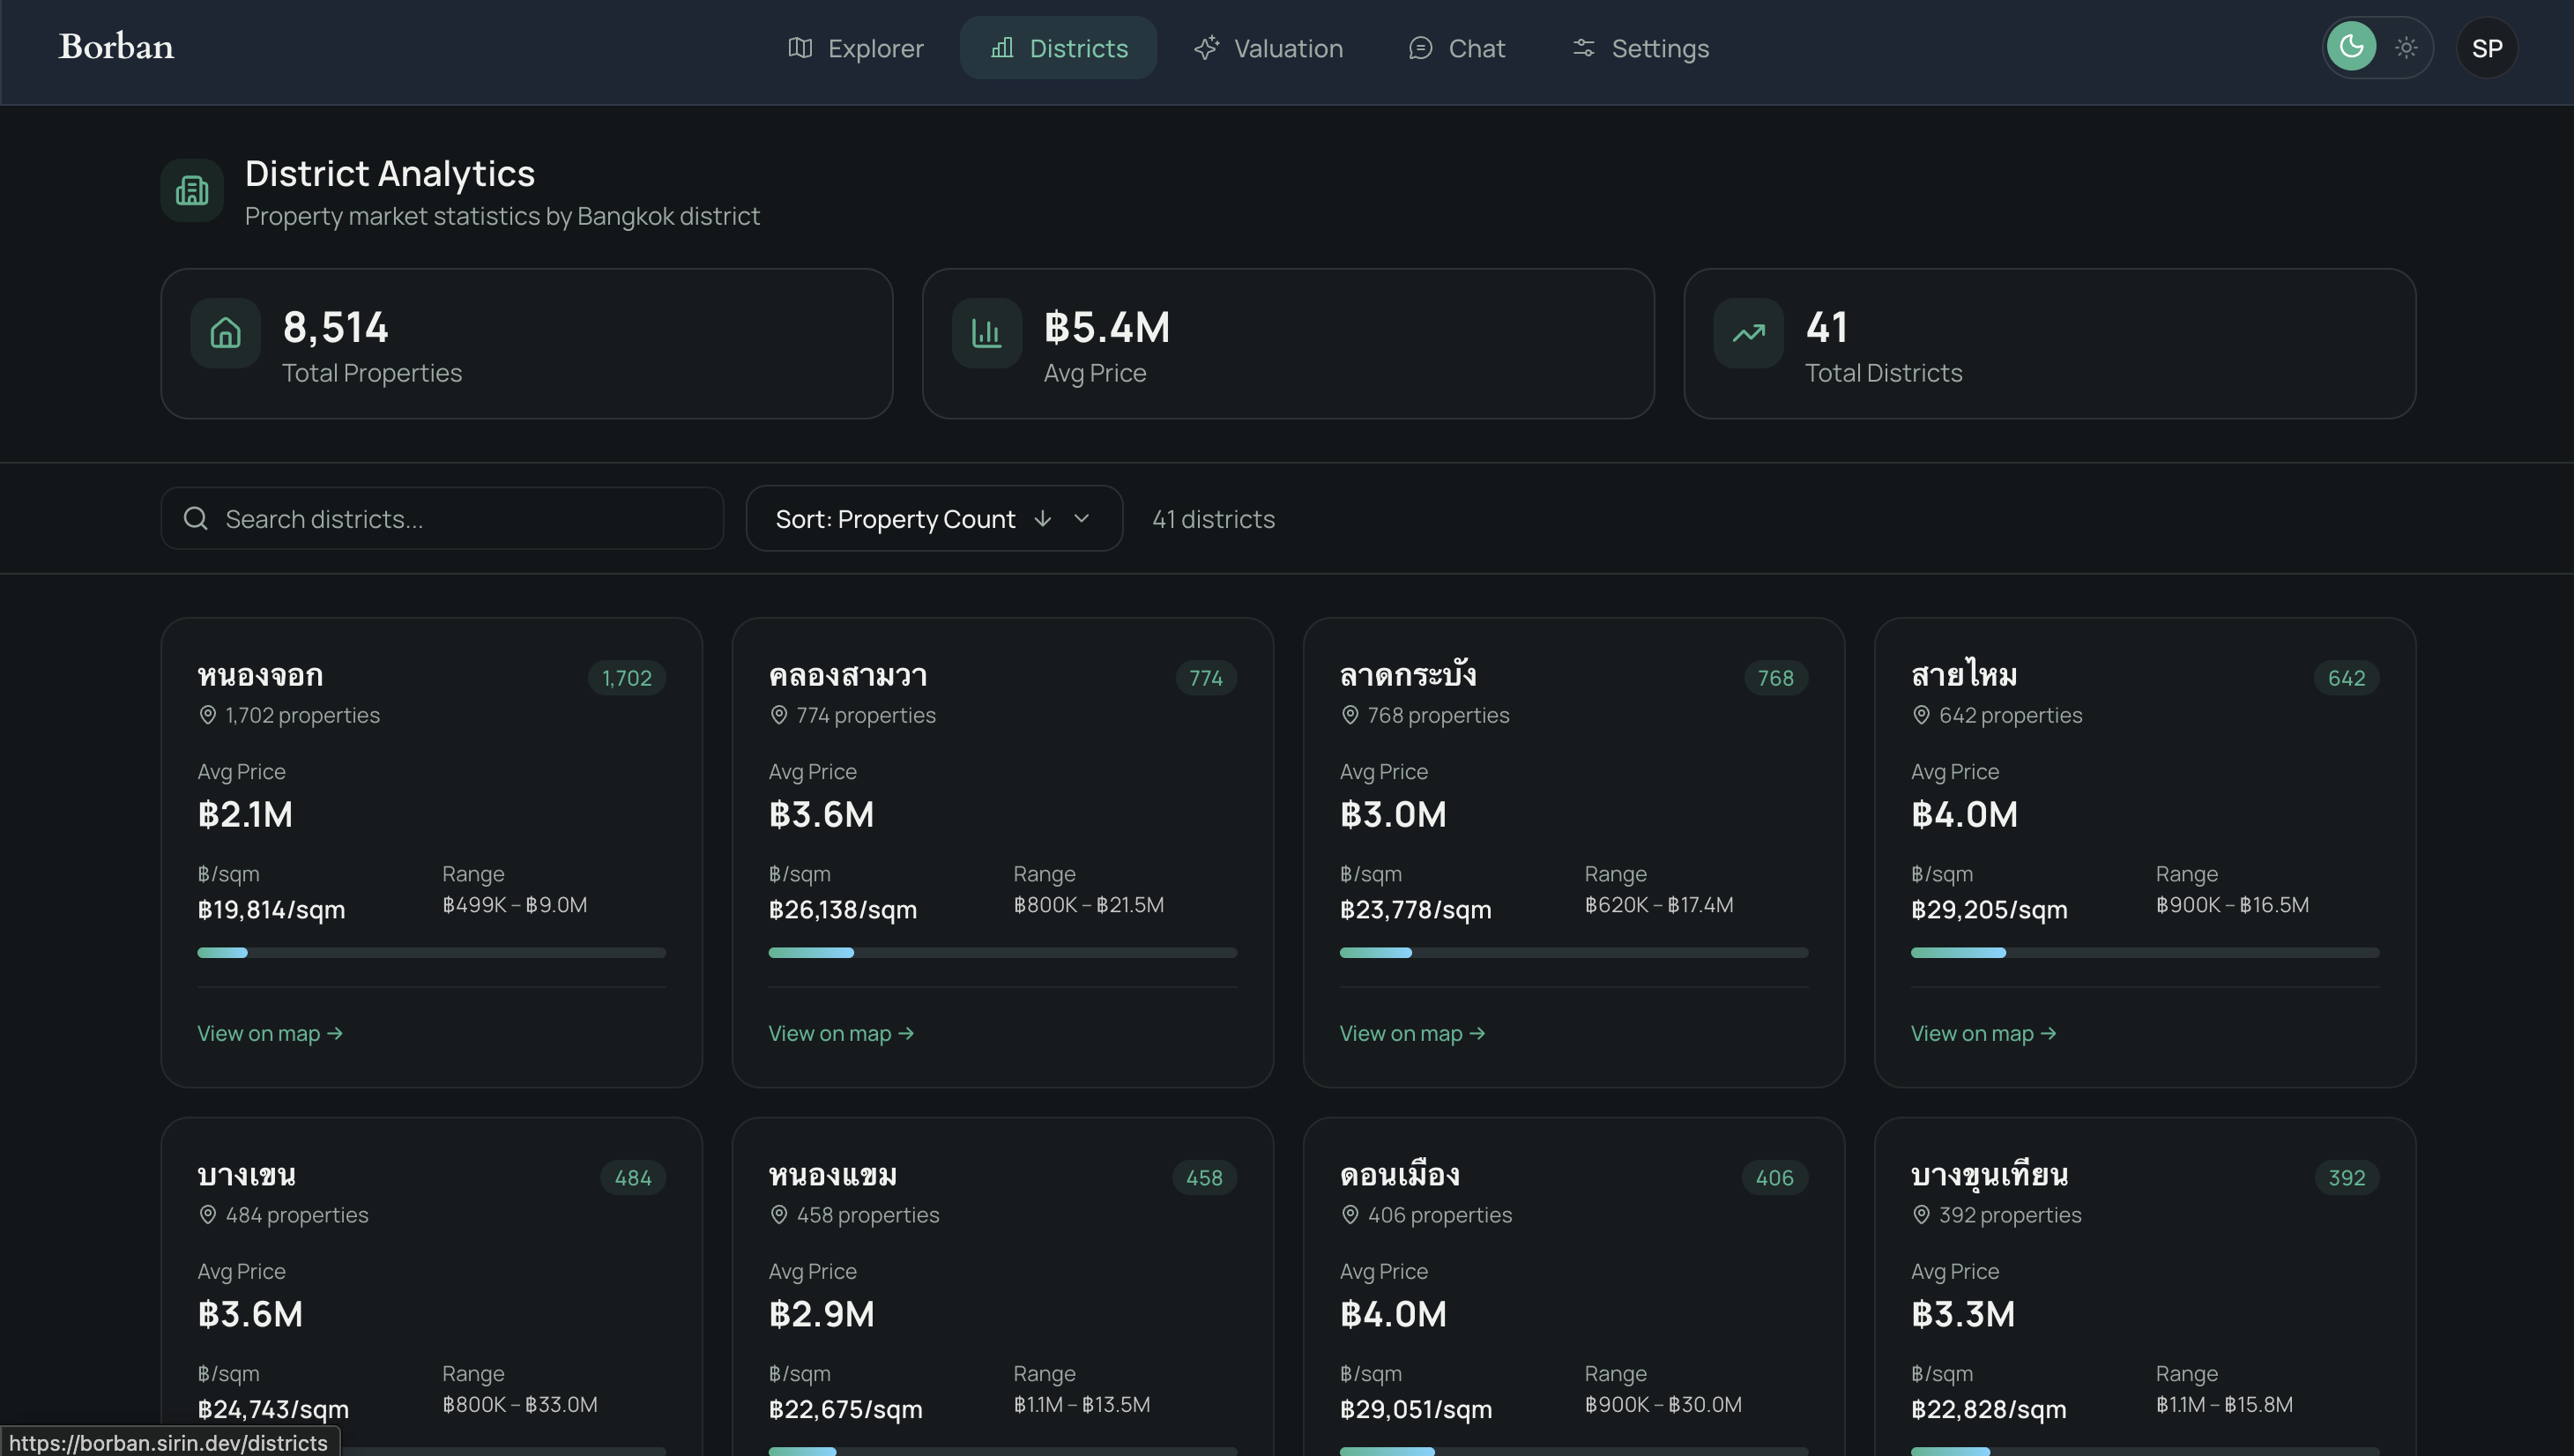
\includegraphics[width=\textwidth]{assets/chapter-7/district-analytic-page.png}
    \caption{District Analytics Page}
    \label{fig:chapter7-district-page}
\end{figure}

\begin{figure}[htbp]
    \centering
    \begin{subfigure}[t]{0.58\textwidth}
        \centering
        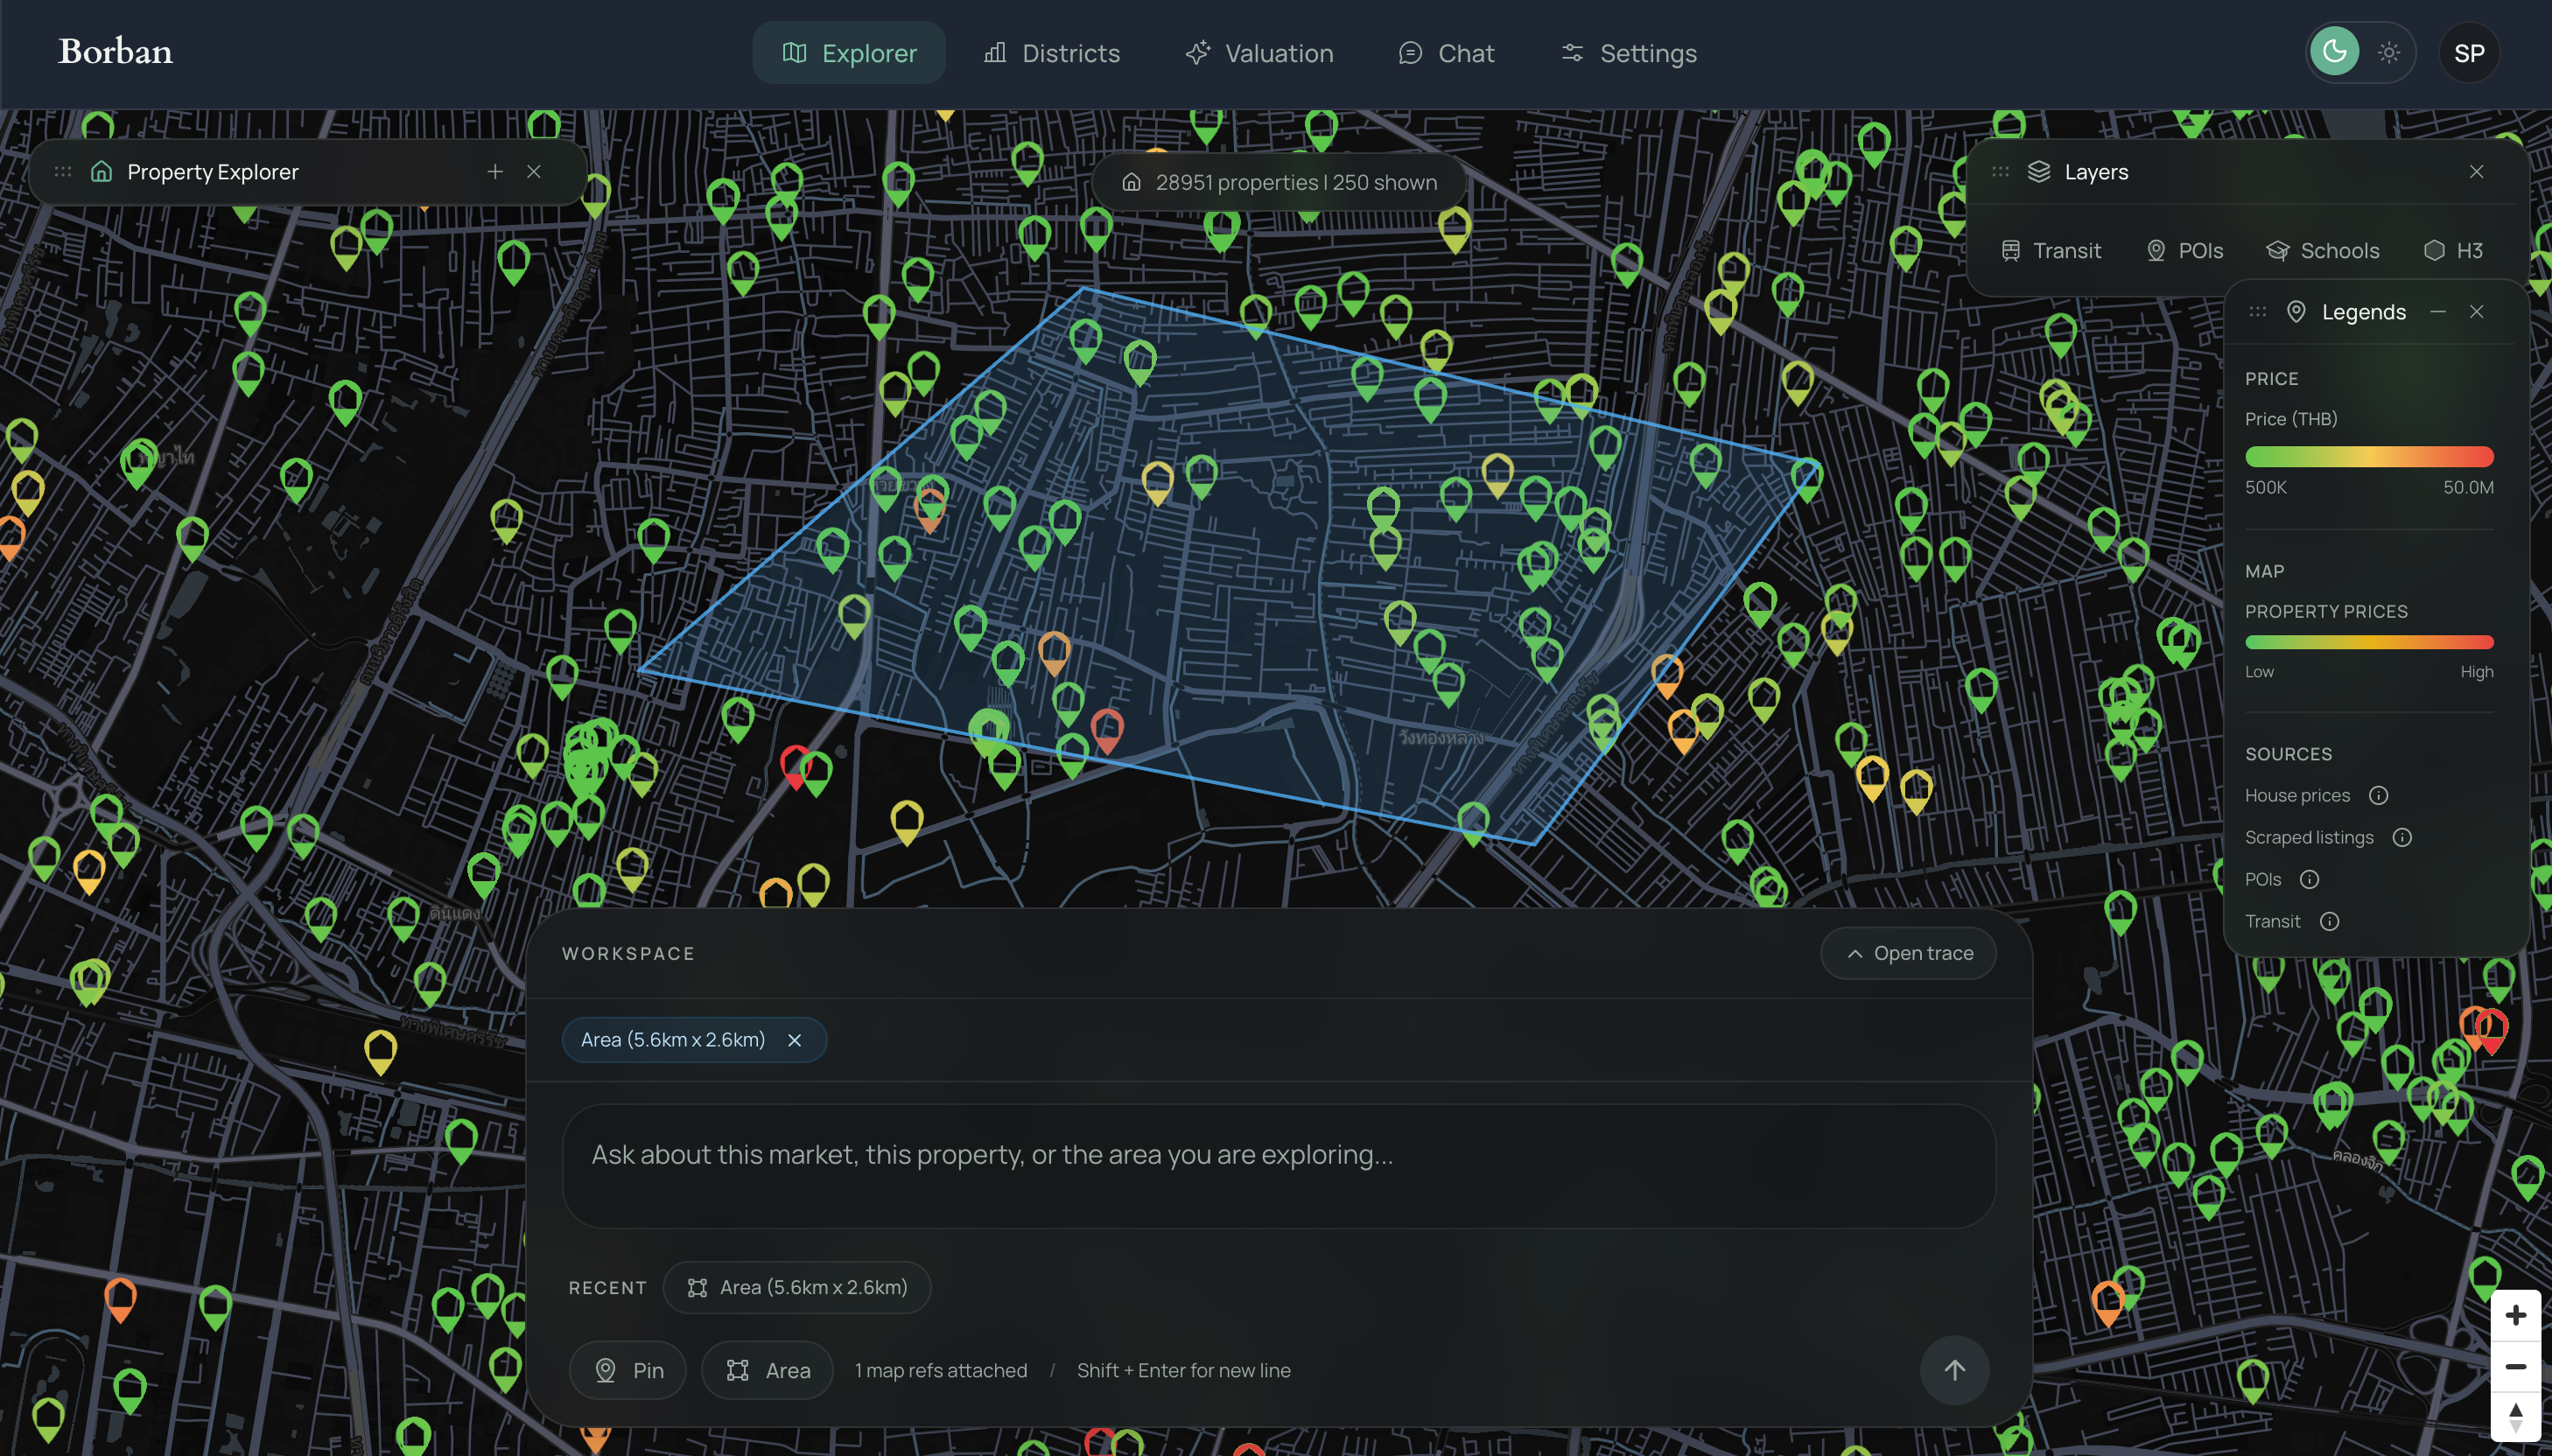
\includegraphics[width=\textwidth]{assets/chapter-7/ai-agent-map.png}
        \caption{Agent-assisted map workspace}
    \end{subfigure}
    \hfill
    \begin{subfigure}[t]{0.37\textwidth}
        \centering
        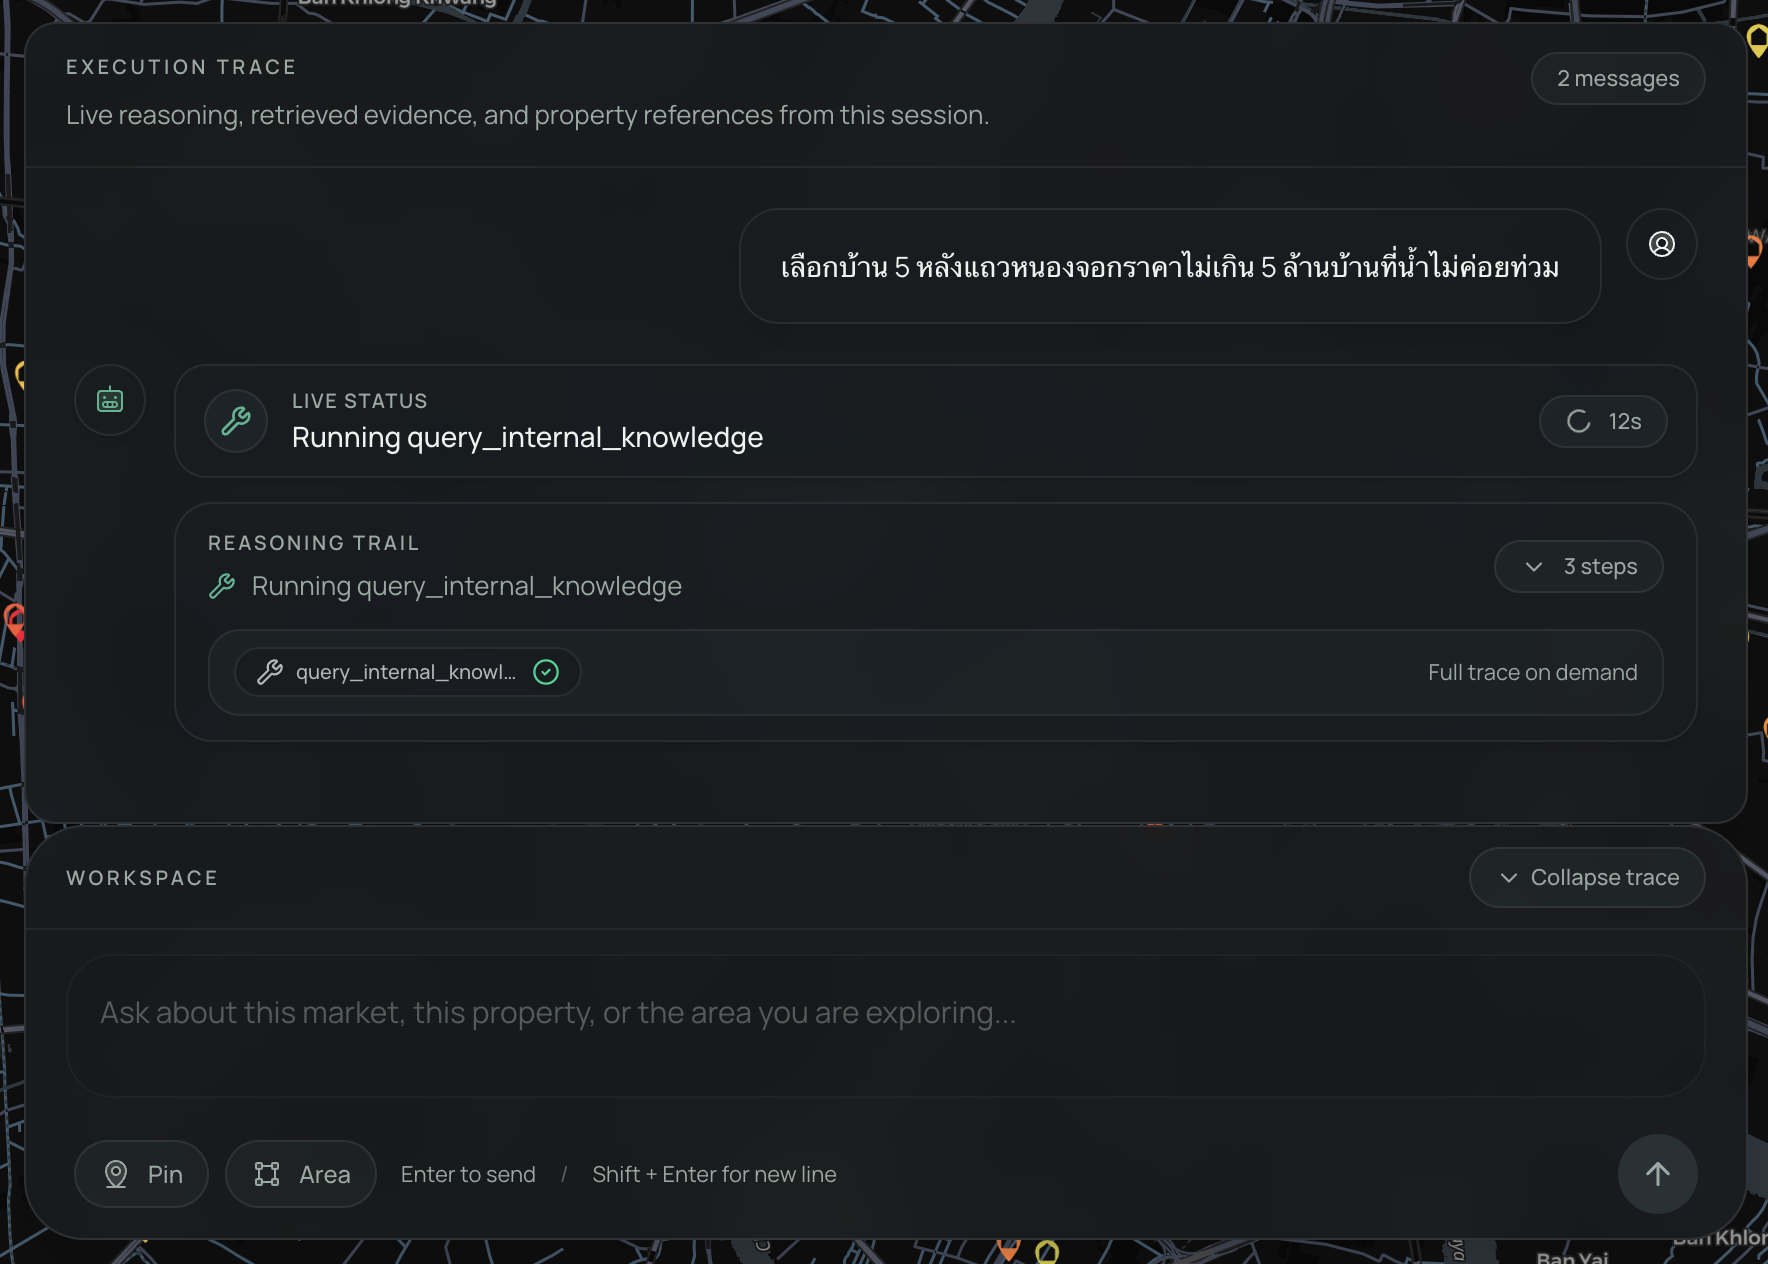
\includegraphics[width=\textwidth]{assets/chapter-7/ai-agent-chat.png}
        \caption{Chat-focused agent interface}
    \end{subfigure}
    \caption{AI Agent Interfaces}
    \label{fig:chapter7-agent-views}
\end{figure}

\clearpage

%----------------------------------------------------------------------
\section{Technical and System Deliverables}
%----------------------------------------------------------------------

In addition to the frontend pages, the project delivers the technical infrastructure required to make the platform operational. These outputs are important because BorBann depends on geospatial queries, AI inference, retrieval support, and operational controls rather than static page rendering alone.

Table \ref{tab:chapter7-technical-deliverables} lists the main backend and operational deliverables. These items are the runtime foundation that allows the frontend workflows to access data, compute analytics, and serve AI-assisted responses.

\begin{table}[htbp]
    \centering
    \small
    \renewcommand{\arraystretch}{1.25}
    \begin{tabularx}{\textwidth}{>{\raggedright\arraybackslash}p{0.21\textwidth}>{\raggedright\arraybackslash}p{0.19\textwidth}>{\raggedright\arraybackslash}X}
        \toprule
        \rowcolor[gray]{0.9} \textbf{Technical Deliverable} & \textbf{Implementation Form} & \textbf{Delivered Function} \\
        \midrule
        Geospatial backend API & FastAPI services & Exposes valuation, chat, location intelligence, listing, and district analytics endpoints. \\
        Spatial database platform & PostgreSQL + PostGIS & Stores and queries property, POI, transit, and district-level geographic data. \\
        Retrieval layer & pgvector and internal knowledge services & Supports evidence-based chatbot responses and location-specific retrieval. \\
        Valuation engine & Production LightGBM path & Returns predicted price, confidence, explanations, district comparison, and H3 context. \\
        Explainability support & SHAP and feature-importance pipeline & Produces local and global factor explanation paths with measurable evaluation support. \\
        Observability package & Metrics and refresh monitoring & Prometheus-compatible metrics, cache indicators, refresh counters, and health signals. \\
        Deployment package & Docker Compose and runbook & Production stack definition, deployment scripts, environment guidance, and rollback support. \\
        CI/CD package & GitHub Actions workflows & Automated test, lint, frontend build, and quality-gate execution. \\
        \bottomrule
    \end{tabularx}
    \caption{Technical Deliverables}
    \label{tab:chapter7-technical-deliverables}
\end{table}

%----------------------------------------------------------------------
\section{Testing and Evaluation Report}
%----------------------------------------------------------------------

The project deliverables include detailed testing and evaluation outputs. These are necessary because BorBann contains multiple layers of functionality: user interface workflows, backend APIs, geospatial analytics, machine learning prediction, and AI-agent behavior.

\subsection{Testing Coverage Summary}

Table \ref{tab:chapter7-testing-coverage} outlines the validation methodologies implemented in the system. It combines automated correctness checks, build validation, agent quality gates, and load-testing evidence.

\begin{table}[htbp]
    \centering
    \small
    \renewcommand{\arraystretch}{1.25}
    \begin{tabularx}{\textwidth}{>{\raggedright\arraybackslash}p{0.19\textwidth}>{\raggedright\arraybackslash}p{0.24\textwidth}>{\raggedright\arraybackslash}X}
        \toprule
        \rowcolor[gray]{0.9} \textbf{Test Area} & \textbf{Representative Coverage} & \textbf{Purpose of Validation} \\
        \midrule
        Backend unit tests & 13 unit test modules covering predictor types, feature contributions, explainability utilities, internal knowledge, and tool planning behavior. & Verify correctness of core service logic before integration. \\
        Backend integration tests & 2 integration modules covering chat status, provider validation, SSE event flow, session handling, attachments, and event ordering. & Confirm that API contracts and end-to-end chat flows work correctly. \\
        Frontend validation & CI frontend job runs dependency install, lint, test, and production build. & Ensure the UI architecture remains robust and complies with project quality standards. \\
        Quality gate checks & Dedicated CI quality-gate job with a 10-case agent benchmark policy. & Prevent unreviewed degradation in chatbot quality when a benchmark report exists. \\
        Load validation & k6 Sprint A reports and optimization follow-up reports. & Measure latency, error rate, cache behavior, and operational bottlenecks under load. \\
        \bottomrule
    \end{tabularx}
    \caption{Testing Coverage Summary}
    \label{tab:chapter7-testing-coverage}
\end{table}

The evaluation phase yielded empirical performance metrics rather than isolated test definitions. The next two tables separate automated validation evidence from performance evidence so that each result remains readable and fits the thesis layout cleanly.

\subsection{Automated Validation Result}

Table \ref{tab:chapter7-automated-testing-results} lists the primary quality assurance checks integrated into the continuous integration pipeline.

\begin{table}[htbp]
    \centering
    \small
    \renewcommand{\arraystretch}{1.25}
    \begin{tabularx}{\textwidth}{>{\raggedright\arraybackslash}p{0.19\textwidth}>{\raggedright\arraybackslash}p{0.18\textwidth}>{\raggedright\arraybackslash}p{0.18\textwidth}>{\raggedright\arraybackslash}X}
        \toprule
        \rowcolor[gray]{0.9} \textbf{Evaluation Item} & \textbf{Method} & \textbf{Observed Result} & \textbf{Interpretation} \\
        \midrule
        CI backend validation & GitHub Actions unit and integration jobs & Automated backend tests run with Python 3.13 and PostGIS service support. & The system delivers a repeatable backend validation flow for both isolated logic and API-level behavior. \\
        CI frontend validation & GitHub Actions frontend job & Frontend pipeline runs dependency install, lint, test, and production build. & The frontend architecture operates as a continuously validated application to ensure robustness. \\
        Chat API contract tests & Integration testing of chat endpoints & Verified SSE content type, session ID return, attachment handling, and event ordering such as thinking-first and done-last behavior. & The chat system includes explicit verification of stream behavior and session-based interaction. \\
        Valuation service tests & Unit testing of prediction components & Baseline predictor types, distance calculations, dataclasses, and predictor registry behavior are tested. & Core valuation service behavior is guarded by repeatable tests before model output is used by the UI. \\
        Golden benchmark quality gate & Ten-case benchmark with score and tool-first requirements & The benchmark requires 100\% tool-first compliance for factual queries and a median judge score of at least 7.0 across 10 cases. & This gives the team a measurable way to identify chatbot weaknesses rather than relying on anecdotal review. \\
        \bottomrule
    \end{tabularx}
    \caption{Automated Validation Results}
    \label{tab:chapter7-automated-testing-results}
\end{table}

\subsection{Performance and Load Result}

Table \ref{tab:chapter7-performance-results} reports the measured performance figures captured during Sprint A load testing and the later tile optimization cycle.

\begin{table}[htbp]
    \centering
    \small
    \renewcommand{\arraystretch}{1.25}
    \begin{tabularx}{\textwidth}{>{\raggedright\arraybackslash}p{0.19\textwidth}>{\raggedright\arraybackslash}p{0.18\textwidth}>{\raggedright\arraybackslash}p{0.18\textwidth}>{\raggedright\arraybackslash}X}
        \toprule
        \rowcolor[gray]{0.9} \textbf{Evaluation Item} & \textbf{Method} & \textbf{Observed Result} & \textbf{Interpretation} \\
        \midrule
        Load test baseline & k6 Sprint A Run F & HTTP request failure rate 0.1590, average latency 15635.48 ms, p95 latency 37167.72 ms, check success 1.0, and 4321 requests over the run. & Stability improved after transit-query and transaction-recovery fixes, but the local profile still misses the intended latency target. \\
        Baseline cache behavior & Post-run observability snapshot for Run F & Listings tile cache hit rate 0.0591, location-intelligence cache hit rate 0.0, and database query errors reduced from 1093 in Run E to 0 in Run F. & The run confirms cleaner backend stability, but cache effectiveness remains uneven across expensive workflows. \\
        Load optimization result & Materialized tile source comparison & Representative mixed-workload performance improved from 1.81\% failed requests and 12.6 s p95 latency to 0.00\% failed requests and 6.63 s p95 latency. & Tile-serving optimization clearly improved reliability and tail latency, even though some non-tile bottlenecks remain. \\
        Tile endpoint spot validation & Functional validation after optimization & Cold tile response was about 46 ms, warm tile response about 2 ms, and refresh duration about 2.7--3.1 s with 1 successful and 0 failed refresh cycles observed. & The optimized tile path is significantly cheaper after caching and materialized-source support. \\
        \bottomrule
    \end{tabularx}
    \caption{Performance and Load Results}
    \label{tab:chapter7-performance-results}
\end{table}

The testing results show two important points. First, BorBann has delivered validation artifacts across functional correctness, interface behavior, and performance. Second, the reports do not hide remaining weaknesses. The chatbot benchmark still requires quality recovery, and some geospatial-heavy workflows remain above the desired latency target in local stress conditions.

%----------------------------------------------------------------------
\section{Model Evaluation Report}
%----------------------------------------------------------------------

The valuation component is one of the main deliverables of the project, so its report must include not only prediction output but also model-selection evidence. The project currently uses the LightGBM-based C5 path as the stable production baseline because it remains more reliable than later C6-family candidates under the accepted benchmark policy.

\subsection{Grouped Benchmark Result Table}

Table \ref{tab:chapter7-model-benchmark-grouped} reports the grouped benchmark results from the canonical benchmark summary. These values show the absolute error and fit metrics used to compare the stable C5 path with later C6-family candidates.

\begin{table}[htbp]
    \centering
    \small
    \renewcommand{\arraystretch}{1.2}
    \begin{tabularx}{\textwidth}{>{\raggedright\arraybackslash}p{0.16\textwidth}>{\raggedright\arraybackslash}p{0.1\textwidth}>{\raggedleft\arraybackslash}p{0.15\textwidth}>{\raggedleft\arraybackslash}p{0.15\textwidth}>{\raggedleft\arraybackslash}p{0.15\textwidth}>{\raggedleft\arraybackslash}p{0.1\textwidth}}
        \toprule
        \rowcolor[gray]{0.9} \textbf{Dataset} & \textbf{Stage} & \textbf{Overall MAE} & \textbf{Treasury MAE} & \textbf{Listing MAE} & \textbf{R\textsuperscript{2}} \\
        \midrule
        clean\_grouped & C5 & 1,006,223 & 802,621 & 4,385,310 & 0.779 \\
        clean\_grouped & C6 & 1,594,915 & 1,297,796 & 6,526,043 & 0.454 \\
        clean\_grouped & C6I & 1,575,586 & 1,280,060 & 6,480,273 & 0.469 \\
        clean\_grouped & C6IR & 1,575,491 & 1,280,060 & 6,478,605 & 0.469 \\
        all\_grouped & C5 & 1,822,393 & 816,535 & 3,334,910 & 0.819 \\
        all\_grouped & C6 & 2,811,255 & 1,304,607 & 5,076,815 & 0.564 \\
        all\_grouped & C6I & 2,835,192 & 1,268,005 & 5,191,786 & 0.571 \\
        all\_grouped & C6IR & 2,835,223 & 1,268,005 & 5,191,864 & 0.571 \\
        \bottomrule
    \end{tabularx}
    \caption{Grouped Model Benchmark Results}
    \label{tab:chapter7-model-benchmark-grouped}
\end{table}

Table \ref{tab:chapter7-model-delta} focuses on the percentage regression against the C5 baseline. These relative values make it easier to explain why later models were not promoted, even when they added more complexity.

\begin{table}[htbp]
    \centering
    \small
    \renewcommand{\arraystretch}{1.2}
    \begin{tabularx}{\textwidth}{>{\raggedright\arraybackslash}p{0.12\textwidth}>{\raggedleft\arraybackslash}p{0.18\textwidth}>{\raggedleft\arraybackslash}p{0.18\textwidth}>{\raggedleft\arraybackslash}p{0.18\textwidth}>{\raggedleft\arraybackslash}X}
        \toprule
        \rowcolor[gray]{0.9} \textbf{Stage} & \textbf{Clean Listing Delta} & \textbf{Clean Treasury Delta} & \textbf{All Listing Delta} & \textbf{All Treasury Delta} \\
        \midrule
        C5 & 0.00\% & 0.00\% & 0.00\% & 0.00\% \\
        C6 & +48.82\% & +61.70\% & +52.23\% & +59.77\% \\
        C6I & +47.78\% & +59.48\% & +55.67\% & +55.29\% \\
        C6IR & +47.74\% & +59.48\% & +55.68\% & +55.29\% \\
        \bottomrule
    \end{tabularx}
    \caption{Regression Against the C5 Baseline}
    \label{tab:chapter7-model-delta}
\end{table}

Table \ref{tab:chapter7-model-time-split} adds the time-split check and the extra XGBoost comparison rows, which together complete the 12 canonical benchmark entries evaluated in the study.

\begin{table}[htbp]
    \centering
    \small
    \renewcommand{\arraystretch}{1.2}
    \begin{tabularx}{\textwidth}{>{\raggedright\arraybackslash}p{0.17\textwidth}>{\raggedright\arraybackslash}p{0.12\textwidth}>{\raggedright\arraybackslash}p{0.1\textwidth}>{\raggedleft\arraybackslash}p{0.15\textwidth}>{\raggedleft\arraybackslash}p{0.15\textwidth}>{\raggedleft\arraybackslash}X}
        \toprule
        \rowcolor[gray]{0.9} \textbf{Dataset} & \textbf{Model} & \textbf{Stage} & \textbf{Overall MAE} & \textbf{Listing MAE} & \textbf{R\textsuperscript{2}} \\
        \midrule
        clean\_time & LightGBM & C5 & 998,152 & 6,862,957 & 0.784 \\
        clean\_time & LightGBM & C6 & 1,318,455 & 10,019,947 & 0.617 \\
        clean\_grouped & XGBoost & C6 & 1,560,390 & 6,462,368 & 0.475 \\
        all\_grouped & XGBoost & C6 & 2,800,799 & 5,128,357 & 0.573 \\
        \bottomrule
    \end{tabularx}
    \caption{Time-Split and Additional Model Rows}
    \label{tab:chapter7-model-time-split}
\end{table}

\subsection{Model Selection Interpretation}

Table \ref{tab:chapter7-model-selection-interpretation} converts the benchmark evidence into a deployment decision. It shows why C5 remains the production baseline even though more experimental variants were also implemented and benchmarked.

\begin{table}[htbp]
    \centering
    \small
    \renewcommand{\arraystretch}{1.25}
    \begin{tabularx}{\textwidth}{>{\raggedright\arraybackslash}p{0.22\textwidth}>{\raggedright\arraybackslash}X>{\raggedright\arraybackslash}p{0.24\textwidth}}
        \toprule
        \rowcolor[gray]{0.9} \textbf{Evaluation Topic} & \textbf{Observed Evidence} & \textbf{Decision} \\
        \midrule
        Baseline stability & C5 shows the best balance between listing accuracy and treasury stability in both clean and all-grouped settings. & Keep C5 as the production-ready model path. \\
        Candidate model regression & C6-family variants regress strongly on listing and treasury MAE compared with C5. & Do not promote C6-family models to production. \\
        Time-split robustness & On the clean time split, C6 remains materially worse than C5 in overall, treasury, and listing MAE. & Avoid replacing the baseline with a weaker time-split performer. \\
        Complexity versus usefulness & More complex variants, including image-augmented branches and HGT research direction, do not currently deliver stronger benchmark results. & Keep advanced models as research outputs, not default deployment models. \\
        Governance and acceptance policy & The system implements explicit acceptance gates based on listing improvement and treasury regression caps. & Model promotion is controlled by benchmark evidence rather than assumption. \\
        \bottomrule
    \end{tabularx}
    \caption{Model Selection Interpretation}
    \label{tab:chapter7-model-selection-interpretation}
\end{table}

\subsection{Explainability Evaluation Summary}

The project also delivers model-explanation support beyond prediction accuracy. The explainability evaluation code reports seven quantitative signals: one SHAP rank-correlation value, two overlap measures (top-5 and top-10), three perturbation-based faithfulness measures, and one expected-feature coverage value. These outputs are important because they provide evidence that the explanation layer is tied to model behavior rather than only visual presentation.

Table \ref{tab:chapter7-explainability-evaluation} summarizes the explainability evaluation package and the measurable checks included in the implementation.

\begin{table}[htbp]
    \centering
    \small
    \renewcommand{\arraystretch}{1.25}
    \begin{tabularx}{\textwidth}{>{\raggedright\arraybackslash}p{0.22\textwidth}>{\raggedright\arraybackslash}p{0.26\textwidth}>{\raggedright\arraybackslash}X}
        \toprule
        \rowcolor[gray]{0.9} \textbf{Explainability Item} & \textbf{Delivered Mechanism} & \textbf{Purpose} \\
        \midrule
        Local explanation & Per-request local SHAP contribution output converted to approximate THB effect. & Show the main request-specific factors affecting the estimate. \\
        Global reference explanation & Gain-based feature-importance summary from the model. & Provide stable model-level signal reference. \\
        Rank agreement check & Spearman rank correlation plus top-5 and top-10 overlap between SHAP and gain rankings. & Verify whether different explanation views remain aligned on important features. \\
        Faithfulness check & Perturbation delta for top-ranked features, random-reference delta, and faithfulness lift. & Test whether important features cause meaningful prediction change. \\
        Expected-feature coverage & Coverage check for expected domain factors such as area and major distance features within the inspected top-k set. & Confirm that important domain features appear in explanation results. \\
        \bottomrule
    \end{tabularx}
    \caption{Explainability Evaluation Deliverables}
    \label{tab:chapter7-explainability-evaluation}
\end{table}

The explainability evaluation was conducted using automated testing procedures to validate the model's interpretation metrics. Table \ref{tab:chapter7-explainability-results} summarizes the performance metrics obtained during this evaluation phase.

\begin{table}[htbp]
    \centering
    \small
    \renewcommand{\arraystretch}{1.25}
    \begin{tabularx}{\textwidth}{>{\raggedright\arraybackslash}p{0.28\textwidth}>{\raggedleft\arraybackslash}p{0.18\textwidth}>{\raggedright\arraybackslash}X}
        \toprule
        \rowcolor[gray]{0.9} \textbf{Metric} & \textbf{Current Result} & \textbf{Interpretation} \\
        \midrule
        SHAP rank correlation & 0.90 & SHAP ranking is strongly aligned with the gain-based global ranking. \\
        Top-5 overlap & 0.80 & Four of the top five important features are shared between the two ranking views. \\
        Faithfulness lift & 1.70$\times$ & Top SHAP-ranked features produce about 1.70 times more prediction change than random features. \\
        Expected-feature coverage & 1.00 & All expected domain features in the tested report are present in the inspected top-ranked set. \\
        \bottomrule
    \end{tabularx}
    \caption{Explainability Evaluation Results}
    \label{tab:chapter7-explainability-results}
\end{table}

Overall, the model evaluation deliverable is not limited to one best score. It includes benchmark tables, model-selection rules, and explanation-evaluation support so that the delivered valuation feature remains both useful and accountable.
